% ============================================================
% M3 S2 导学件·波1 臂5 片件 —— 课时16 2.7.2抛物线的几何性质（50键＝探究45＋评价46—50）
% 生成：M3 成卷轮 S2 波1 臂5｜2026-09-14｜编译 cwd＝本目录（中文路径禁 \input 绝对路径）
%   xelatex main-true.tex ×2 → 含详解印本；xelatex main-false.tex ×2 → 纯题版（单源双本）
% 输入链（全只读）：题面库 课时16-2.7.2抛物线性质.md（题面逐字装配）＋ -答案侧.md（值逐字回嵌）
%   ＋ 定稿/批D-课时16-2.7.2抛物线性质.md（详解回嵌源：§七 补产全文区＋件末「导学 G5 补产」）；
%   toolchain＝qp-m3.sty（钉后版 md5 7c3930362be8a0a2bdf21bbf8ac16573，本地挂载副本，破损即停）。
% 母版：课时01-坐标法（结构骨架照抄）；门谱：工作区/_tmpM3S2波1臂5_0914/门谱/。
% 键账：件内 ansblock 键集 ≡ 题面库片键集 ≡ manifest 键序（50 键，零缺漏零多余）；
%   印面号 1—50＝探究 1—45＋课堂评价 46—50，键↔号映射见 值台账-课时16.json；
%   让位席拓16-18 以无键留块（键集豁免登记在案），拓键实幅 01~30 且 18 不占键。
% 括线判据（派单承重墙，禁放宽）：估高＞8 行（wlen（全角1·ASCII0.5，剔\命令）/23 栏宽字口径，
%   est＝ceil）→ 括线模（{\ansblockgrayfalse 包装}），否则灰底；逐键读数入值台账。
% 值快照：50 键值均与答案侧「值：」行逐字全等（零换算；− 走 preamble 路由、p̃ 正文安全已探针实证）。
% 印面符号口径（0914 S6 销案承军师案一·文句化）：对勾/叉号印面改「成立/相符/不合」文语，
%   直箭头/双横箭头印面改「得/即/故/等价于」文语（pifont 路由退场）；∥、∈、≤、≥、≡、路由减号等照台账渲染注记不变。
% ============================================================
\documentclass[fontset=none]{ctexart}
\usepackage{qp-m3}
% —— 印面逐字符号路由补钉（探针实证 0914：书宋缺 U+2212/U+2013，▱ 诸字库皆缺→NSC 子块；
%     禁改 sty 本体保 md5；对勾/叉号原探针实证走 pifont 路由（0914 S6 文句化后印面退场） ——
\usepackage{pifont}%
\xeCJKDeclareCharClass{Default}{"2212}%
\xeCJKDeclareCharClass{Default}{"2013}%
\setCJKfamilyfont{nscblk}[Path=C:/提示词/工作区/字替对照-0909/variantF/fonts/,BoldFont=NSC-w600.ttf]{NSC-w500.ttf}%
\xeCJKDeclareSubCJKBlock{nscblk}{"25B1}%
\newcommand{\pxparallelogram}{{\CJKfamily{nscblk}▱}}%
% —— 断行微调（CJK 胶 0.10em 母版同款；拉伸 plus 0.08→0.30em 实证校准 0914：窄栏详解
%     长公式链行亏 5—40pt，0.08em 拉伸点稀（数学边界无 CJK 胶）吸不住→badness 10000 必报
%     underfull（\emergencystretch 与降 rel/binop 罚均救不了，报告按打包线实胶重算）；
%     0.30em 后亏量全数吸收，自然齐行零漂移；探针 probe6—8 实证） ——
\xeCJKsetup{CJKglue={\hskip 0.10em plus 0.30em minus 0.05em}}%
% —— 页脚件名（qp-headfoot 复用入口） ——
\renewcommand{\qpzhangming}{第二章\quad 平面解析几何}%
\renewcommand{\qpjianming}{导学件}%

\begin{document}

\zhangtitle{第二章\quad 平面解析几何}
\jietitle{2.7.2 抛物线的几何性质}
\mubiaoline
\mubiaomu{1}{掌握抛物线的范围、对称性、顶点、离心率及焦点、准线、通径等几何性质，能由方程读出性质、由性质定方程；}
\mubiaomu{2}{会用抛物线的定义实现焦半径与点到准线距离的互化，解决距离最值、焦点弦与定值等问题；}
\mubiaomu{3}{经历“由形究数、由数判形”的过程，体会抛物线与椭圆、双曲线研究路径的一致性，发展直观想象与逻辑推理素养.}

\vspace{1.7mm}
\begin{multicols}{2}
\emergencystretch=1em

% ============================================================
% 课前预习（知识点导学填空；零键零答案——预习键位按检查口令④裁定前口径，
% \kongbai{} 空线＋\zhentib 判断题面形，两档等形不泄答）
% ============================================================
\huaxing{课}{前}{预}{习}{知识导学\quad 素养初识}

\zsd{一}{抛物线的标准方程与几何性质}

\tiaomu{1}{抛物线 \(y^{2}=2px\)（\(p>0\)）的焦点坐标为\kongbai{}，准线方程为\kongbai{}，其中 \(p\) 的几何意义是\kongbai{}．\zhuzhu{焦点在开口方向正向 \(p/2\) 处，准线在反向 \(p/2\) 处；\(p\) 是焦点到准线的距离，四种标准形通用.}}

\tiaomu{2}{抛物线 \(y^{2}=2px\)（\(p>0\)）的范围是\kongbai{}，对称轴为\kongbai{}，顶点是\kongbai{}，离心率 \(e=\)\kongbai{}；过焦点且垂直于对称轴的弦（通径）的长为\kongbai{}．\zhuzhu{抛物线的离心率恒为 1；通径 \(2p\) 越大开口越开阔，是比较两抛物线开口大小的尺子.}}

\zsd{二}{焦半径与定义互化}

\tiaomu{1}{抛物线上一点 \(P\) 到焦点的距离，等于它到\kongbai{} 的距离；对 \(y^{2}=2px\)（\(p>0\)）上的点 \(P(x_{0},y_{0})\)，焦半径 \(|PF|=\)\kongbai{}．\zhuzhu{焦半径与到准线距离的互化是抛物线最值、焦点弦问题的第一工具，注意开口方向决定符号.}}

\zhenhead{判断正误(正确的打\gou{},错误的打\cha{})}

\zhentib{(1)}{抛物线上的点到焦点的距离与它到准线的距离相等．}

\zhentib{(2)}{抛物线的离心率随开口变大而变大．}

\liubai[9mm]{此处书写}

% ============================================================
% 课中探究（考点探究〔例+变式〕＝练/拓槽 45 键；题后紧跟答案＝ansblock 内嵌，
% 值照答案侧逐字，详解承批D回嵌＋印面清洗：〔…〕审计尾注剔除、印面符号文句化（0914 S6 销案追记））
% ============================================================
\huaxing{课}{中}{探}{究}{考点探究\quad 素养小结}

% ---------- 探究点一 性质辨析与焦点准线直用 ----------
\tjdnr{一}{性质辨析与焦点准线直用}{例\textbf{1}}{简单(知识点一)}{求抛物线 \(y^{2}=8x\) 的焦点到直线 \(x-\sqrt{3}y=0\) 的距离．}
\xiexwei{7mm}

\begin{ansblock}[2章-练-课时16-04]
% ans:2章-练-课时16-04
\ansitem{1}{1}
\ansnote{详解}{\(2p=8\)、\(p=4\)，焦点 \(F(2,0)\)．由点到直线的距离公式，\(d=|2-\sqrt{3}\times 0|/\sqrt{1^{2}+(\sqrt{3})^{2}}=2/\sqrt{4}=1\)．}
\end{ansblock}

\liB{变式\textbf{2}}{简单(知识点一)}{}{求下列方程表示的抛物线的焦点坐标和准线方程：}

\bindp (1) \(y^{2}-6x=0\)；　(2) \(x^{2}+10y=0\)；

\bindp (3) \(y=(3/8)x^{2}\)；　(4) \(ax+y^{2}=0\)（\(a\neq 0\)）．
\xiexwei{7mm}

{\ansblockgrayfalse
\begin{ansblock}[2章-练-课时16-03]
% ans:2章-练-课时16-03
\ansitem{2}{(1) 焦点(3/2,0)，准线 x=−3/2；(2) 焦点(0,−5/2)，准线 y=5/2；(3) 焦点(0,2/3)，准线 y=−2/3；(4) 焦点(−a/4,0)，准线 x=a/4}
\ansnote{详解}{(1) \(y^{2}=6x\)：\(2p=6\)、\(p=3\)，开口向右，焦点 \((p/2,0)=(3/2,0)\)，准线 \(x=-3/2\)．(2) \(x^{2}=-10y\)：\(2p=10\)、\(p=5\)，开口向下，焦点 \((0,-5/2)\)，准线 \(y=5/2\)．(3) \(x^{2}=(8/3)y\)：\(2p=8/3\)、\(p=4/3\)，开口向上，焦点 \((0,2/3)\)，准线 \(y=-2/3\)．(4) \(y^{2}=-ax\)（\(a\neq 0\)）：一次项系数为 \(-a\)，无论 \(a>0\)（开口向左）或 \(a<0\)（开口向右），焦点均为 \((-a/4,0)\)、准线均为 \(x=a/4\)（\(a>0\) 时焦点在 \(x\) 轴负半轴，\(a<0\) 时在正半轴，公式统一）．}
\end{ansblock}}

\liB{变式\textbf{3}}{简单(知识点一)}{\duoxuan\hspace{0.6em}}{关于抛物线 \(y^{2}=-2x\)，下列说法正确的是\nobreak(\kongwei)}

\lxopt{A．开口向左}

\lxopt{B．焦点坐标为\((-1,0)\)}

\lxopt{C．准线为 \(x=1\)}

\lxopt{D．对称轴为 \(x\) 轴}

\begin{ansblock}[2章-练-课时16-01]
% ans:2章-练-课时16-01
\ansitem{3}{AD}
\ansnote{详解}{对照标准形 \(y^{2}=-2px\)（\(p>0\)）：\(2p=2\)、\(p=1\)，一次项系数为负，开口向左，A 正确；焦点为 \((-p/2,0)=(-1/2,0)\)，B 所给 \((-1,0)\) 错（把 \(p\) 误作 \(p/2\)）；准线为 \(x=p/2=1/2\)，C 所给 \(x=1\) 错；对称轴为 \(x\) 轴，D 正确．故选：AD．}
\end{ansblock}

\tjdnr{一}{性质辨析与焦点准线直用}{例\textbf{4}}{简单(知识点二)}{设抛物线 \(y^{2}=8x\) 上一点 \(P\) 到 \(y\) 轴的距离是 4，求点 \(P\) 到该抛物线焦点的距离．}
\xiexwei{7mm}

\begin{ansblock}[2章-练-课时16-05]
% ans:2章-练-课时16-05
\ansitem{4}{6}
\ansnote{详解}{\(y^{2}=8x\) 中 \(2p=8\)、\(p=4\)，准线 \(x=-2\)．点 \(P\) 到 \(y\) 轴距离为 4，而抛物线上点横坐标 \(x\geqslant 0\)，故 \(x_{P}=4\)．由定义，\(P\) 到焦点的距离等于 \(P\) 到准线的距离：\(|PF|=x_{P}+p/2=4+2=6\)．（校验：\(P(4,\pm 4\sqrt{2})\)，\(|PF|=\sqrt{(4-2)^{2}+32}=\sqrt{36}=6\)，回验相符．）}
\end{ansblock}

\liB{变式\textbf{5}}{简单(知识点二)}{}{已知抛物线 \(y=4x^{2}\) 上的一点 \(M\) 的纵坐标为 1，求点 \(M\) 到焦点的距离．}
\xiexwei{7mm}

\begin{ansblock}[2章-练-课时16-02]
% ans:2章-练-课时16-02
\ansitem{5}{17/16}
\ansnote{详解}{化标准形：\(y=4x^{2}\) 即 \(x^{2}=(1/4)y\)，故 \(2p=1/4\)、\(p=1/8\)，焦点 \(F(0,1/16)\)，准线 \(y=-1/16\)．由抛物线定义，点 \(M\) 到焦点的距离等于它到准线的距离，\(|MF|=y_{M}+p/2=1+1/16=17/16\)．（回代校验：\(x_{M}^{2}=1/4\)、\(M(\pm 1/2,1)\)，\(|MF|^{2}=x_{M}^{2}+(y_{M}-1/16)^{2}=1/4+225/256=289/256\)，\(|MF|=17/16\)，回验相符．）}
\end{ansblock}

\liB{变式\textbf{6}}{简单(知识点二)}{}{若抛物线 \(y^{2}=2px\)（\(p>0\)）上一点 \(M\) 到焦点 \(F\) 的距离 \(|MF|=2p\)，求点 \(M\) 的坐标．}
\xiexwei{7mm}

\begin{ansblock}[2章-练-课时16-06]
% ans:2章-练-课时16-06
\ansitem{6}{M(3p/2, ±√3 p)}
\ansnote{详解}{设 \(M(x_{0},y_{0})\)，\(x_{0}\geqslant 0\)．由定义，\(|MF|\) 等于 \(M\) 到准线 \(x=-p/2\) 的距离，即 \(x_{0}+p/2=2p\)，得 \(x_{0}=3p/2\)．代入方程：\(y_{0}^{2}=2p\cdot(3p/2)=3p^{2}\)，\(y_{0}=\pm\sqrt{3}p\)．故 \(M(3p/2,\sqrt{3}p)\) 或 \(M(3p/2,-\sqrt{3}p)\)．}
\end{ansblock}

\tjdnr{一}{性质辨析与焦点准线直用}{例\textbf{7}}{简单(知识点一)}{已知抛物线的顶点在坐标原点，对称轴是坐标轴，且过点 \(P(-2,2\sqrt{2})\)，求抛物线的标准方程．}
\xiexwei{7mm}

\begin{ansblock}[2章-练-课时16-07]
% ans:2章-练-课时16-07
\ansitem{7}{y²=−4x 或 x²=√2 y}
\ansnote{详解}{\(P(-2,2\sqrt{2})\) 在第二象限，开口只可能向左或向上．情形一，对称轴为 \(x\) 轴：设 \(y^{2}=-2px\)（\(p>0\)），代入得 \((2\sqrt{2})^{2}=-2p\cdot(-2)=4p\)、\(p=2\)，即 \(y^{2}=-4x\)．情形二，对称轴为 \(y\) 轴：设 \(x^{2}=2py\)（\(p>0\)），代入得 \(4=2p\cdot 2\sqrt{2}\)、\(2p=\sqrt{2}\)，即 \(x^{2}=\sqrt{2}y\)．（回验：\(8=-4\times(-2)\)，成立；\(4=\sqrt{2}\times 2\sqrt{2}\)，成立．）}
\end{ansblock}

\liB{变式\textbf{8}}{简单(知识点一)}{}{若抛物线 \(y^{2}=2px\)（\(p>0\)）的焦点与椭圆 \(x^{2}/6+y^{2}/2=1\) 的右焦点重合，求 \(p\) 的值．}
\xiexwei{7mm}

\begin{ansblock}[2章-练-课时16-08]
% ans:2章-练-课时16-08
\ansitem{8}{p=4}
\ansnote{详解}{椭圆中 \(c^{2}=6-2=4\)，右焦点 \((2,0)\)．抛物线焦点 \((p/2,0)\)，由 \(p/2=2\) 得 \(p=4\)．}
\end{ansblock}

\liB{变式\textbf{9}}{简单(知识点一)}{}{以 \(x\) 轴为对称轴，抛物线通径的长为 8，顶点在坐标原点的抛物线的方程是\nobreak(\kongwei)}

\bindopt {\fontsize{10.5pt}{\qpTJgLeadLiti}\selectfont \makebox[\dimexpr0.5\linewidth-1em\relax][l]{A．\(y^{2}=8x\)}\makebox[\dimexpr0.5\linewidth-1em\relax][l]{B．\(y^{2}=-8x\)}\par}

\bindopt {\fontsize{10.5pt}{\qpTJgLeadLiti}\selectfont \makebox[\dimexpr0.5\linewidth-1em\relax][l]{C．\(y^{2}=8x\) 或 \(y^{2}=-8x\)}\makebox[\dimexpr0.5\linewidth-1em\relax][l]{D．\(x^{2}=8y\) 或 \(x^{2}=-8y\)}\par}

\begin{ansblock}[2章-练-课时16-10]
% ans:2章-练-课时16-10
\ansitem{9}{C}
\ansnote{详解}{顶点在原点、对称轴为 \(x\) 轴，方程形如 \(y^{2}=\pm 2px\)（\(p>0\)）．通径（过焦点且垂直于对称轴的弦）长为 \(2p\)，由 \(2p=8\) 得 \(p=4\)，故方程为 \(y^{2}=8x\)（焦点在 \(x\) 轴正半轴）或 \(y^{2}=-8x\)（焦点在负半轴），两向各一，选 C．（排除 D：其对称轴为 \(y\) 轴．）}
\end{ansblock}

\xiaojie{①识别：凡由方程读性质（开口、焦点、准线、通径）、或由性质（过定点、焦点重合）反定方程的题，判归本题型.}
\bindp {\kaishu ②操作：先化标准形定开口与 \(p\)，焦点 \((\pm p/2,0)\)、准线 \(x=\mp p/2\) 直写；开口待定时按对称轴分类讨论，解出后回代检验.}
\bindp {\kaishu ③收束：焦半径＝到准线的距离，符号随开口方向定；通径 \(2p\) 是比较开口大小的尺子.}

% ---------- 探究点二 焦点弦、最值与压轴 ----------
\tjdnr{二}{焦点弦、最值与压轴}{例\textbf{10}}{简单(知识点三)}{已知抛物线 \(C\)：\(y^{2}=x\) 的焦点为 \(F\)，过点 \(F\) 且斜率为 \(\sqrt{3}\) 的直线交抛物线 \(C\) 于 \(A\)、\(B\) 两点，则 \(|AF|\cdot|BF|\) 等于\nobreak(\kongwei)}

\bindopt {\fontsize{10.5pt}{\qpTJgLeadLiti}\selectfont \makebox[\dimexpr0.25\linewidth-0.5em\relax][l]{A．\(1/3\)}\makebox[\dimexpr0.25\linewidth-0.5em\relax][l]{B．\(4/3\)}\makebox[\dimexpr0.25\linewidth-0.5em\relax][l]{C．\(1\)}\makebox[\dimexpr0.25\linewidth-0.5em\relax][l]{D．\(4\)}\par}

\begin{ansblock}[2章-练-课时16-09]
% ans:2章-练-课时16-09
\ansitem{10}{A（1/3）}
\ansnote{详解}{\(y^{2}=x\) 中 \(2p=1\)，焦点 \(F(1/4,0)\)，准线 \(x=-1/4\)．直线 \(l\)：\(y=\sqrt{3}(x-1/4)\)．代入 \(y^{2}=x\) 得 \(3(x-1/4)^{2}=x\)，整理为 \(48x^{2}-40x+3=0\)，故 \(x_{1}+x_{2}=40/48=5/6\)，\(x_{1}x_{2}=3/48=1/16\)．由定义，\(|AF|=x_{1}+1/4\)、\(|BF|=x_{2}+1/4\)，\(|AF|\cdot|BF|=x_{1}x_{2}+(1/4)(x_{1}+x_{2})+1/16=1/16+5/24+1/16=16/48=1/3\)．故选 A．}
\end{ansblock}

\liB{变式\textbf{11}}{中档(知识点三)}{}{已知 \(F\) 为抛物线 \(C\)：\(y^{2}=4x\) 的焦点，过点 \(F\) 的直线 \(l\) 交抛物线 \(C\) 于 \(A\)，\(B\) 两点．若 \(|AB|=8\)，则线段 \(AB\) 的中点 \(M\) 到直线 \(x+1=0\) 的距离为\nobreak(\kongwei)}

\bindopt {\fontsize{10.5pt}{\qpTJgLeadLiti}\selectfont \makebox[\dimexpr0.25\linewidth-0.5em\relax][l]{A．\(2\)}\makebox[\dimexpr0.25\linewidth-0.5em\relax][l]{B．\(4\)}\makebox[\dimexpr0.25\linewidth-0.5em\relax][l]{C．\(8\)}\makebox[\dimexpr0.25\linewidth-0.5em\relax][l]{D．\(16\)}\par}

\begin{ansblock}[2章-练-课时16-11]
% ans:2章-练-课时16-11
\ansitem{11}{B}
\ansnote{详解}{\(y^{2}=4x\) 的焦点 \(F(1,0)\)，准线 \(x=-1\)，即直线 \(x+1=0\)．分别过 \(A\)、\(B\)、\(M\) 作准线的垂线，垂足为 \(C\)、\(D\)、\(N\)．由定义，\(|AC|=|AF|\)、\(|BD|=|BF|\)，故 \(|AC|+|BD|=|AF|+|BF|=|AB|=8\)．又 \(AC\parallel MN\parallel BD\) 且 \(M\) 为 \(AB\) 中点，\(MN\) 为直角梯形 \(ABDC\) 的中位线，\(|MN|=(|AC|+|BD|)/2=4\)，即点 \(M\) 到准线 \(x=-1\) 的距离为 4．故选：B．}
\end{ansblock}

\tjdnr{二}{焦点弦、最值与压轴}{例\textbf{12}}{中档(知识点二)}{已知抛物线的方程为 \(x^{2}=8y\)，\(F\) 是其焦点，点 \(A(-2,4)\) 在抛物线的内部，在此抛物线上求一点 \(P\)，使 \(|PF|+|PA|\) 的值最小．}
\xiexwei{7mm}

{\ansblockgrayfalse
\begin{ansblock}[2章-练-课时16-12]
% ans:2章-练-课时16-12
\ansitem{12}{P(−2,1/2)（最小值 6）}
\ansnote{详解}{\(x^{2}=8y\) 的准线为 \(l\)：\(y=-2\)．设 \(P\) 在 \(l\) 上的射影为 \(Q\)，过 \(A\) 作 \(AB\perp l\) 于 \(B\)，则 \(|AB|=y_{A}-(-2)=4+2=6\)．由定义 \(|PF|=|PQ|\)，故 \(|PF|+|PA|=|PQ|+|PA|\geqslant|AQ|\geqslant|AB|=6\)：第一个不等号当 \(A\)、\(P\)、\(Q\) 共线（\(P\) 与 \(A\) 同取横坐标 \(-2\)）时取等，第二个不等号当 \(Q\) 与 \(B\) 重合时取等，两条件同时满足．把 \(x=-2\) 代入 \(x^{2}=8y\) 得 \(y=1/2\)，故所求点 \(P(-2,1/2)\)，此时 \((|PF|+|PA|)_{\min}=|AB|=y_{A}+2=6\)．}
\end{ansblock}}

\liB{变式\textbf{13}}{中档(知识点二)}{}{已知抛物线 \(y^{2}=16x\) 和点 \(A(4,0)\)，点 \(M\) 在此抛物线上运动，求点 \(M\) 到点 \(A\) 的距离的最小值，并指出取得最小值时点 \(M\) 的坐标．}
\xiexwei{7mm}

\begin{ansblock}[2章-练-课时16-13]
% ans:2章-练-课时16-13
\ansitem{13}{|MA| 的最小值为 4，此时 M(0,0)}
\ansnote{详解}{设 \(M(x,y)\)，则 \(x\geqslant 0\)，\(y^{2}=16x\)．\par\noindent \(|MA|^{2}=(x-4)^{2}+y^{2}=(x-4)^{2}+16x=x^{2}+8x+16=(x+4)^{2}\)．\par\noindent 由 \(x\geqslant 0\) 得 \((x+4)^{2}\geqslant 16\)，当且仅当 \(x=0\) 时等号成立，此时 \(y=0\)，\(|MA|_{\min}=4\)，\(M(0,0)\)．（注：\(2p=16\)、\(p/2=4\)，\(A(4,0)\) 恰为该抛物线的焦点，\(|MA|=|MF|=x+4\geqslant 4\) 与配方路径互证．）}
\end{ansblock}

\tjdnr{二}{焦点弦、最值与压轴}{例\textbf{14}}{中档(知识点三)}{正三角形的一个顶点位于坐标原点，另外两个顶点在抛物线 \(y^{2}=2px\)（\(p>0\)）上，求这个正三角形的边长．}
\xiexwei{12mm}

{\ansblockgrayfalse
\begin{ansblock}[2章-练-课时16-14]
% ans:2章-练-课时16-14
\ansitem{14}{4√3 p}
\ansnote{详解}{设正三角形 \(OAB\) 的顶点 \(A(x_{1},y_{1})\)、\(B(x_{2},y_{2})\) 在抛物线上，则 \(y_{1}^{2}=2px_{1}\)、\(y_{2}^{2}=2px_{2}\)．由 \(|OA|=|OB|\) 得 \(x_{1}^{2}+y_{1}^{2}=x_{2}^{2}+y_{2}^{2}\)，即 \((x_{1}^{2}-x_{2}^{2})+2p(x_{1}-x_{2})=0\)，\((x_{1}-x_{2})(x_{1}+x_{2}+2p)=0\)．因 \(x_{1}\geqslant 0\)、\(x_{2}\geqslant 0\) 且 \(2p>0\)（若 \(x_{1}\)、\(x_{2}\) 之一为 0 则三角形退化），括号第二因子为正，故 \(x_{1}=x_{2}\)，从而 \(y_{2}=-y_{1}\neq 0\)，线段 \(AB\) 关于 \(x\) 轴对称．\(x\) 轴垂直平分 \(AB\) 且平分 \(\angle AOB\)，\(\angle AOx=30^{\circ}\)，故 \(y_{1}/x_{1}=\tan 30^{\circ}=\sqrt{3}/3\)、\(x_{1}=\sqrt{3}y_{1}\)．代入 \(y_{1}^{2}=2p\cdot\sqrt{3}y_{1}\) 得 \(y_{1}=2\sqrt{3}p\)，边长 \(|AB|=2y_{1}=4\sqrt{3}p\)．}
\end{ansblock}}

\liB{变式\textbf{15}}{难(知识点三)}{}{已知 \(O\) 为坐标原点，过抛物线 \(y^{2}=2px\)（\(p>0\)）的焦点 \(F\) 作一条倾斜角为 \(\pi/4\) 的直线，与抛物线相交于 \(A\)，\(B\) 两点．}

\bindp (1) 用 \(p\) 表示 \(A\)，\(B\) 之间的距离；

\bindp (2) 证明：\(\cos\angle AOB\) 的大小是与 \(p\) 无关的定值，并求出这个值．
\xiexwei{18mm}

{\ansblockgrayfalse
\begin{ansblock}[2章-练-课时16-15]
% ans:2章-练-课时16-15
\ansitem{15}{(1) |AB|=4p；(2) 定值 cos∠AOB=−3√41/41（与 p 无关）}
\ansnote{详解}{(1) 过 \(F(p/2,0)\)、倾斜角 \(\pi/4\) 的直线为 \(y=x-p/2\)．代入 \(y^{2}=2px\)：\((x-p/2)^{2}=2px\)，即 \(x^{2}-3px+p^{2}/4=0\)（\(\Delta=9p^{2}-p^{2}=8p^{2}>0\)）．设 \(A(x_{A},y_{A})\)、\(B(x_{B},y_{B})\)，则 \(x_{A}+x_{B}=3p\)，\(x_{A}x_{B}=p^{2}/4\)．由定义（焦半径），\par\noindent \(|AB|=|AF|+|BF|=(x_{A}+p/2)+(x_{B}+p/2)=x_{A}+x_{B}+p=4p\)．\par\noindent (2) 该弦所在直线与 \(x\) 轴交于 \(F\)，两端点 \(A\)、\(B\) 分居 \(x\) 轴两侧，纵坐标一正一负，其积为负：\par\noindent \(y_{A}y_{B}=(x_{A}-p/2)(x_{B}-p/2)=x_{A}x_{B}-(p/2)(x_{A}+x_{B})+p^{2}/4=p^{2}/4-3p^{2}/2+p^{2}/4=-p^{2}\)（与焦点弦结论 \(y_{1}y_{2}=-p^{2}\) 相符，此即符号判据）．\par\noindent 于是 \(x_{A}x_{B}+y_{A}y_{B}=p^{2}/4-p^{2}=-3p^{2}/4\)．又 \(|OA|^{2}=x_{A}^{2}+y_{A}^{2}=x_{A}^{2}+2px_{A}=x_{A}(x_{A}+2p)\)，同理 \(|OB|^{2}=x_{B}(x_{B}+2p)\)．\par\noindent 故 \(|OA|\cdot|OB|=\sqrt{x_{A}x_{B}}\cdot\sqrt{x_{A}x_{B}+2p(x_{A}+x_{B})+4p^{2}}=(p/2)\cdot\sqrt{p^{2}/4+6p^{2}+4p^{2}}=(p/2)\cdot(\sqrt{41}/2)p=\sqrt{41}p^{2}/4\)．\par\noindent 在 \(\triangle AOB\) 中由余弦定理，\(\cos\angle AOB=(|OA|^{2}+|OB|^{2}-|AB|^{2})/(2|OA|\cdot|OB|)\)．\par\noindent 而 \(|OA|^{2}+|OB|^{2}-|AB|^{2}=(x_{A}-x_{B})^{2}+(y_{A}-y_{B})^{2}=2(x_{A}x_{B}+y_{A}y_{B})=-3p^{2}/2\)，\par\noindent 故 \(\cos\angle AOB=(-3p^{2}/4)/(\sqrt{41}p^{2}/4)=-3/\sqrt{41}\)，分母有理化得 \(-3\sqrt{41}/41\)，\(p^{2}\) 全部约去，与 \(p\) 无关．}
\end{ansblock}}

\liB{变式\textbf{16}}{难(知识点三)}{}{过抛物线 \(C\)：\(x^{2}=4y\) 的焦点 \(F\) 作斜率分别为 \(k_{1}\)、\(k_{2}\) 的两条直线 \(l_{1}\)、\(l_{2}\)，其中 \(l_{1}\) 交抛物线 \(C\) 于 \(A\)、\(B\) 两点，\(l_{2}\) 交抛物线 \(C\) 于 \(D\)、\(E\) 两点．若 \(k_{1}k_{2}=-2\)，求 \(|AB|+|DE|\) 的最小值．}
\xiexwei{18mm}

{\ansblockgrayfalse
\begin{ansblock}[2章-练-课时16-16]
% ans:2章-练-课时16-16
\ansitem{16}{24}
\ansnote{详解}{\(x^{2}=4y\) 的焦点 \(F(0,1)\)，准线 \(y=-1\)，抛物线上点之焦半径 \(|AF|=y_{A}+1\)（到准线距离，焦半径公式见例 36）．\(l_{1}\)：\(y=k_{1}x+1\) 代入 \(x^{2}=4y\) 得 \(x^{2}-4k_{1}x-4=0\)（\(\Delta=16k_{1}^{2}+16>0\) 恒成立）．设 \(A(x_{1},y_{1})\)、\(B(x_{2},y_{2})\)，则 \(x_{1}+x_{2}=4k_{1}\)，\(y_{1}+y_{2}=k_{1}(x_{1}+x_{2})+2=4k_{1}^{2}+2\)．于是 \par\noindent \(|AB|=|AF|+|BF|=(y_{1}+1)+(y_{2}+1)=y_{1}+y_{2}+2=4k_{1}^{2}+4\)．\par\noindent 同理 \(|DE|=4k_{2}^{2}+4\)．故 \par\noindent \(|AB|+|DE|=4(k_{1}^{2}+k_{2}^{2})+8\geqslant 8|k_{1}k_{2}|+8=8\times 2+8=24\)，\par\noindent 当且仅当 \(|k_{1}|=|k_{2}|\) 且 \(k_{1}k_{2}=-2\)，即 \((k_{1},k_{2})=(\sqrt{2},-\sqrt{2})\) 或 \((-\sqrt{2},\sqrt{2})\) 时等号成立．所求最小值为 24．}
\end{ansblock}}

\xiaojie{①识别：凡过焦点的弦长、弦中点距离、焦半径最值、正三角形（对称型）与弦长定值问题，判归本题型.}
\bindp {\kaishu ②操作：焦半径用定义 \(|PF|=x_{P}+p/2\) 化为坐标和；焦点弦先联立韦达，纵（横）坐标和差积配入弦长或焦半径公式.}
\bindp {\kaishu ③收束：最值优先想定义转化（射影、三点共线取等）；对称型抓“对称轴垂直平分弦”；定值证明把参数约净并回代特位核对.}

% ---------- 探究点三 拓展·定义转化与最值 ----------
\tjdnr{三}{拓展·定义转化与最值}{例\textbf{17}}{中档(知识点一)}{已知点 \((x,y)\) 在抛物线 \(y^{2}=4x\) 上，则 \(z=x^{2}+(1/2)y^{2}+3\) 的最小值是\nobreak(\kongwei)}

\bindopt {\fontsize{10.5pt}{\qpTJgLeadLiti}\selectfont \makebox[\dimexpr0.25\linewidth-0.5em\relax][l]{A．\(2\)}\makebox[\dimexpr0.25\linewidth-0.5em\relax][l]{B．\(3\)}\makebox[\dimexpr0.25\linewidth-0.5em\relax][l]{C．\(4\)}\makebox[\dimexpr0.25\linewidth-0.5em\relax][l]{D．\(0\)}\par}

\begin{ansblock}[2章-拓-课时16-01]
% ans:2章-拓-课时16-01
\ansitem{17}{B}
\ansnote{详解}{点在 \(y^{2}=4x\) 上，故 \(x\geqslant 0\) 且 \(y^{2}=4x\)．代入得 \(z=x^{2}+(1/2)\cdot 4x+3=x^{2}+2x+3=(x+1)^{2}+2\)．由 \(x\geqslant 0\)，\(x=0\) 时 \(z\) 最小，最小值为 3．故选：B．}
\end{ansblock}

\liB{变式\textbf{18}}{中档(知识点二)}{}{已知点 \(P\) 是抛物线 \(x^{2}=4y\) 上的动点，点 \(P\) 在 \(x\) 轴上的射影是点 \(Q\)，点 \(A\) 的坐标是 \((8,7)\)，则 \(|PA|+|PQ|\) 的最小值为\nobreak(\kongwei)}

\bindopt {\fontsize{10.5pt}{\qpTJgLeadLiti}\selectfont \makebox[\dimexpr0.25\linewidth-0.5em\relax][l]{A．\(7\)}\makebox[\dimexpr0.25\linewidth-0.5em\relax][l]{B．\(8\)}\makebox[\dimexpr0.25\linewidth-0.5em\relax][l]{C．\(9\)}\makebox[\dimexpr0.25\linewidth-0.5em\relax][l]{D．\(10\)}\par}

\begin{ansblock}[2章-拓-课时16-03]
% ans:2章-拓-课时16-03
\ansitem{18}{C}
\ansnote{详解}{\(x^{2}=4y\) 的焦点 \(F(0,1)\)，准线 \(y=-1\)．延长 \(QP\) 交准线于 \(M\)，则 \(|PM|=y_{P}+1=|PQ|+1\)；由定义 \(|PM|=|PF|\)，故 \(|PQ|=|PF|-1\)．于是 \par\noindent \(|PA|+|PQ|=|PA|+|PF|-1\geqslant|AF|-1=\sqrt{8^{2}+(7-1)^{2}}-1=10-1=9\)，\par\noindent 当且仅当 \(A\)、\(P\)、\(F\) 三点共线时取等（\(A(8,7)\) 在抛物线外：\(64>4\times 7=28\)，线段 \(AF\) 与抛物线相交，取等可行）．最小值为 9，选 C．}
\end{ansblock}

\liB{变式\textbf{19}}{中档(知识点二)}{}{已知点 \(P(m,n)\) 是抛物线 \(y=-(1/4)x^{2}\) 上一动点，则 \(\sqrt{m^{2}+(n+1)^{2}}+\sqrt{(m-4)^{2}+(n+5)^{2}}\) 的最小值为\nobreak(\kongwei)}

\bindopt {\fontsize{10.5pt}{\qpTJgLeadLiti}\selectfont \makebox[\dimexpr0.25\linewidth-0.5em\relax][l]{A．\(4\)}\makebox[\dimexpr0.25\linewidth-0.5em\relax][l]{B．\(5\)}\makebox[\dimexpr0.25\linewidth-0.5em\relax][l]{C．\(\sqrt{30}\)}\makebox[\dimexpr0.25\linewidth-0.5em\relax][l]{D．\(6\)}\par}

{\ansblockgrayfalse
\begin{ansblock}[2章-拓-课时16-04]
% ans:2章-拓-课时16-04
\ansitem{19}{D}
\ansnote{详解}{化标准形 \(x^{2}=-4y\)：焦点 \(F(0,-1)\)，准线 \(l\)：\(y=1\)．第一根式是 \(P\) 到 \(F(0,-1)\) 的距离 \(|PF|\)，第二根式是 \(P\) 到 \(A(4,-5)\) 的距离 \(|PA|\)．由定义，\(|PF|\) 等于 \(P\) 到准线 \(y=1\) 的距离（\(n\leqslant 0\)，即 \(1-n\)），故 \(|PF|+|PA|\) 不小于 \(A\) 到准线的垂线段长 \(1-(-5)=6\)（\(A\) 在抛物线内部：\(4^{2}=16<-4\times(-5)=20\)，核成立，\(P\) 取垂线段与抛物线交点即可取等）．最小值 6，选 D．}
\end{ansblock}}

\tjdnr{三}{拓展·定义转化与最值}{例\textbf{20}}{中档(知识点二)}{点 \(M(20,40)\)，抛物线 \(y^{2}=2px\)（\(p>0\)）的焦点为 \(F\)，若对于抛物线上的任意点 \(P\)，\(|PM|+|PF|\) 的最小值为 41，则 \(p\) 的值等于\kongbai{}．}
\xiexwei{7mm}

{\ansblockgrayfalse
\begin{ansblock}[2章-拓-课时16-02]
% ans:2章-拓-课时16-02
\ansitem{20}{42 或 22}
\ansnote{详解}{按 \(M\) 与抛物线的位置分类．(1) \(M\) 在抛物线内部或上：\(40^{2}\leqslant 2p\cdot 20\)，即 \(p\geqslant 40\)．设 \(P\) 在准线 \(x=-p/2\) 上的射影为 \(D\)，\(|PF|=|PD|\)，\(M\)、\(P\)、\(D\) 共线时取最小，最小值为 \(M\) 到准线的距离 \(20+p/2=41\)，得 \(p=42\)（\(40\leqslant 42\)，成立）．(2) \(M\) 在抛物线外部：\(p<40\)，\(P\)、\(M\)、\(F\) 共线时取最小，最小值为 \par\noindent \(|MF|=\sqrt{40^{2}+(20-p/2)^{2}}=41\)，\((20-p/2)^{2}=81\)、\(p/2=11\) 或 \(29\)，\(p=22\) 或 \(p=58\)（\(58>40\) 与外部前提矛盾，舍）．\par\noindent 综上 \(p=42\) 或 \(22\)．}
\end{ansblock}}

\liB{变式\textbf{21}}{简单(知识点二)}{}{已知抛物线 \(y^{2}=2x\) 的焦点是 \(F\)，点 \(P\) 是抛物线上的动点，若 \(A(3,2)\)，则 \(|PA|+|PF|\) 的最小值为\kongbai{}，此时点 \(P\) 的坐标为\kongbai{}．}
\xiexwei{7mm}

\begin{ansblock}[2章-拓-课时16-21]
% ans:2章-拓-课时16-21
\ansitem{21}{7/2；P(2,2)}
\ansnote{详解}{\(A(3,2)\)：\(2^{2}=4<2\times 3=6\)，\(A\) 在抛物线内部．准线 \(l\)：\(x=-1/2\)．设 \(P\) 在 \(l\) 上的射影为 \(Q\)，由定义 \(|PF|=|PQ|\)，\(|PA|+|PF|=|PA|+|PQ|\geqslant A\) 到准线的水平距离 \(=3-(-1/2)=7/2\)，当 \(A\)、\(P\)、\(Q\) 共线（\(y_{P}=y_{A}=2\)）时取等．代入 \(y^{2}=2x\) 得 \(x=2\)，即 \(P(2,2)\)，最小值 \(7/2\)．}
\end{ansblock}

\liB{变式\textbf{22}}{中档(知识点三)}{}{已知点 \(A(2,0)\)，\(B(4,0)\)，动点 \(P\) 在抛物线 \(y^{2}=-4x\) 上运动，则使 \(\overrightarrow{AP}\cdot\overrightarrow{BP}\) 取得最小值的点 \(P\) 的坐标是\kongbai{}．}
\xiexwei{7mm}

\begin{ansblock}[2章-拓-课时16-09]
% ans:2章-拓-课时16-09
\ansitem{22}{(0,0)（最小值 8）}
\ansnote{详解}{设 \(P(x_{0},y_{0})\)，\(y_{0}^{2}=-4x_{0}\)（\(x_{0}\leqslant 0\)）．\par\noindent \(\overrightarrow{AP}\cdot\overrightarrow{BP}=(x_{0}-2)(x_{0}-4)+y_{0}^{2}=x_{0}^{2}-6x_{0}+8-4x_{0}=x_{0}^{2}-10x_{0}+8=(x_{0}-5)^{2}-17\)．\par\noindent 由 \(x_{0}\leqslant 0\)，\((x_{0}-5)^{2}\geqslant 25\) 且随 \(x_{0}\) 增大而减小，故 \(x_{0}=0\) 时 \(\overrightarrow{AP}\cdot\overrightarrow{BP}\) 最小，最小值 8，此时 \(y_{0}=0\)，点 \(P(0,0)\)．}
\end{ansblock}

\tjdnr{三}{拓展·定义转化与最值}{例\textbf{23}}{简单(知识点二)}{已知抛物线 \(y^{2}=4x\) 的焦点为 \(F\)，点 \(P(m,-4)\) 在抛物线上，则 \(PF\) 的长为\nobreak(\kongwei)}

\bindopt {\fontsize{10.5pt}{\qpTJgLeadLiti}\selectfont \makebox[\dimexpr0.25\linewidth-0.5em\relax][l]{A．\(2\)}\makebox[\dimexpr0.25\linewidth-0.5em\relax][l]{B．\(3\)}\makebox[\dimexpr0.25\linewidth-0.5em\relax][l]{C．\(4\)}\makebox[\dimexpr0.25\linewidth-0.5em\relax][l]{D．\(5\)}\par}

\begin{ansblock}[2章-拓-课时16-22]
% ans:2章-拓-课时16-22
\ansitem{23}{D}
\ansnote{详解}{\(P\) 在抛物线上：\(16=4m\)、\(m=4\)，\(P(4,-4)\)．焦半径（定义）：准线 \(x=-1\)，\(|PF|=x_{P}+1=4+1=5\)．（两点距复核：\(F(1,0)\)，\(|PF|=\sqrt{9+16}=5\)，回验相符．）选 D．}
\end{ansblock}

\liB{变式\textbf{24}}{中档(知识点三)}{}{已知点 \(P\) 为抛物线 \(y^{2}=4x\) 上一动点，\(A(1,0)\)，\(B(3,0)\)，则 \(\angle APB\) 的最大值为\nobreak(\kongwei)}

\bindopt {\fontsize{10.5pt}{\qpTJgLeadLiti}\selectfont \makebox[\dimexpr0.25\linewidth-0.5em\relax][l]{A．\(\pi/6\)}\makebox[\dimexpr0.25\linewidth-0.5em\relax][l]{B．\(\pi/4\)}\makebox[\dimexpr0.25\linewidth-0.5em\relax][l]{C．\(\pi/3\)}\makebox[\dimexpr0.25\linewidth-0.5em\relax][l]{D．\(\pi/2\)}\par}

{\ansblockgrayfalse
\begin{ansblock}[2章-拓-课时16-06]
% ans:2章-拓-课时16-06
\ansitem{24}{B}
\ansnote{详解}{由对称性不妨设 \(P(x,y)\)（\(y>0\)）．特殊位：\(x=1\) 时 \(P(1,2)\)，\(PA\perp x\) 轴，\(\tan\angle APB=|AB|/|PA|=2/2=1\)，\(\angle APB=\pi/4\)；\(x=3\) 时 \(P(3,2\sqrt{3})\)，\(PB\perp x\) 轴，\(\tan\angle APB=|AB|/|PB|=2/(2\sqrt{3})=\sqrt{3}/3\)，\(\angle APB=\pi/6\)．一般位 \(x\neq 1\) 且 \(x\neq 3\)：\par\noindent \(\tan\angle APB=(k_{PB}-k_{PA})/(1+k_{PA}\cdot k_{PB})\)，其中 \(k_{PA}=y/(x-1)\)、\(k_{PB}=y/(x-3)\)，代入化简得 \(\tan\angle APB=2y/(x^{2}-4x+3+y^{2})\)；\par\noindent 以 \(y^{2}=4x\) 代 \(x=y^{2}/4\)：\(\tan\angle APB=2y/(y^{4}/16+3)=2/((1/16)y^{3}+3/y)=2/((1/16)y^{3}+1/y+1/y+1/y)\)．\par\noindent 分母四项用均值不等式：\((1/16)y^{3}+1/y+1/y+1/y\geqslant 4\sqrt[4]{(1/16)y^{3}\cdot(1/y)^{3}}=4\cdot(1/16)^{1/4}=2\)，故 \(\tan\angle APB\leqslant 2/2=1\)；等号要求 \((1/16)y^{3}=1/y\) 即 \(y=2\)（\(P(1,2)\)，落在 \(x=1\) 特殊位，不在一般位内），故一般位 \(0<\tan\angle APB<1\)、\(0<\angle APB<\pi/4\)．综上 \(\angle APB\) 最大值 \(\pi/4\)，选 B．}
\end{ansblock}}

\liB{变式\textbf{25}}{中档(知识点三)}{}{已知 \(A(2,0)\)，\(B(6,0)\)，\(|BM|=2\)，点 \(N\) 在抛物线 \(y^{2}=8x\) 上，则 \(|MN|+(1/2)|MA|\) 的最小值为\nobreak(\kongwei)}

\bindopt {\fontsize{10.5pt}{\qpTJgLeadLiti}\selectfont \makebox[\dimexpr0.25\linewidth-0.5em\relax][l]{A．\(6\)}\makebox[\dimexpr0.25\linewidth-0.5em\relax][l]{B．\(2\sqrt{5}\)}\makebox[\dimexpr0.25\linewidth-0.5em\relax][l]{C．\(5\)}\makebox[\dimexpr0.25\linewidth-0.5em\relax][l]{D．\(2\sqrt{6}\)}\par}

{\ansblockgrayfalse
\begin{ansblock}[2章-拓-课时16-05]
% ans:2章-拓-课时16-05
\ansitem{25}{D}
\ansnote{详解}{\(M(x,y)\) 在以 \(B(6,0)\) 为圆心、2 为半径的圆上：\((x-6)^{2}+y^{2}=4\)；\(N(x_{0},y_{0})\) 满足 \(y_{0}^{2}=8x_{0}\)（\(x_{0}\geqslant 0\)）．在圆约束下加权配凑：\par\noindent \((1/4)|MA|^{2}=(1/4)[(x-2)^{2}+y^{2}]=(1/4)[(x-2)^{2}+y^{2}]+(3/4)[(x-6)^{2}+y^{2}-4]=(x-5)^{2}+y^{2}\)（所加项在圆上为 0），即 \((1/2)|MA|=|MC|\)，其中 \(C(5,0)\)．\par\noindent 于是 \(|MN|+(1/2)|MA|=|MN|+|MC|\geqslant|CN|\)．\par\noindent 又 \(|CN|^{2}=(x_{0}-5)^{2}+y_{0}^{2}\)，代入 \(y_{0}^{2}=8x_{0}\) 得 \(|CN|^{2}=(x_{0}-1)^{2}+24\geqslant 24\)，即 \(|CN|\geqslant 2\sqrt{6}\)，当且仅当 \(x_{0}=1\)（\(N(1,\pm 2\sqrt{2})\)）且 \(C\)、\(M\)、\(N\) 三点共线（\(M\) 为线段 \(CN\) 与圆的交点）时取等——取等可行：\(C(5,0)\) 在圆内（\(|CB|=1<2\)）而 \(N\) 在圆外（\(|NB|^{2}=(x_{0}-6)^{2}+8x_{0}=(x_{0}-2)^{2}+32>4\) 恒成立），线段 \(CN\) 必与圆相交．最小值 \(2\sqrt{6}\)，选 D．}
\end{ansblock}}

\xiaojie{①识别：凡抛物线上的点与定点（焦点、准线、直线、圆）之间的距离和、乘积最值问题，判归本题型.}
\bindp {\kaishu ②操作：先把双根式识别成“到焦点距离＋到准线（定点）距离”，用定义拉直；圆约束配凑系数（阿氏圆型）化 \(k|MA|\) 为定圆弦.}
\bindp {\kaishu ③收束：取等条件落到三点共线并回代验证可行性（内部分离、交点存在）；目标含参的按位置（内部/外部）分类解.}

% ---------- 探究点四 拓展·焦点弦与定值 ----------
\tjdnr{四}{拓展·焦点弦与定值}{例\textbf{26}}{简单(知识点二)}{设抛物线的顶点为 \(O\)，焦点为 \(F\)，准线为 \(l\)，\(P\) 是抛物线上异于 \(O\) 的一点，过 \(P\) 作 \(PQ\perp l\) 于 \(Q\)．则线段 \(FQ\) 的垂直平分线\nobreak(\kongwei)}

\bindopt {\fontsize{10.5pt}{\qpTJgLeadLiti}\selectfont \makebox[\dimexpr0.5\linewidth-1em\relax][l]{A．经过点 \(O\)}\makebox[\dimexpr0.5\linewidth-1em\relax][l]{B．经过点 \(P\)}\par}

\bindopt {\fontsize{10.5pt}{\qpTJgLeadLiti}\selectfont \makebox[\dimexpr0.5\linewidth-1em\relax][l]{C．平行于直线 \(OP\)}\makebox[\dimexpr0.5\linewidth-1em\relax][l]{D．垂直于直线 \(OP\)}\par}

\begin{ansblock}[2章-拓-课时16-19]
% ans:2章-拓-课时16-19
\ansitem{26}{B}
\ansnote{详解}{连接 \(PF\)．由抛物线定义，\(P\) 到焦点的距离等于 \(P\) 到准线的距离，即 \(|PF|=|PQ|\)，\(\triangle QPF\) 为等腰三角形，\(P\) 到线段 \(FQ\) 两端点等距，故 \(P\) 在线段 \(FQ\) 的垂直平分线上，选 B．（反例排 A：取 \(y^{2}=4x\)、\(P(1,2)\)，则 \(F(1,0)\)、\(Q(-1,2)\)，\(|OF|=1\) 而 \(|OQ|=\sqrt{5}\)，\(O\) 不在垂直平分线上；C、D 随之不恒成立．）}
\end{ansblock}

\liB{变式\textbf{27}}{中档(知识点三)}{\duoxuan\hspace{0.6em}}{已知抛物线 \(C\)：\(y^{2}=2px\)（\(p>0\)）的焦点为 \(F\)，直线 \(l\) 的斜率为 \(\sqrt{3}\) 且经过点 \(F\)，直线 \(l\) 与抛物线 \(C\) 交于点 \(A\)、\(B\) 两点（点 \(A\) 在第一象限），与抛物线的准线交于点 \(D\)，若 \(|AF|=8\)，则以下结论正确的是\nobreak(\kongwei)}

\bindopt {\fontsize{10.5pt}{\qpTJgLeadLiti}\selectfont \makebox[\dimexpr0.5\linewidth-1em\relax][l]{A．\(p=4\)}\makebox[\dimexpr0.5\linewidth-1em\relax][l]{B．\(DF=FA\)}\par}

\bindopt {\fontsize{10.5pt}{\qpTJgLeadLiti}\selectfont \makebox[\dimexpr0.5\linewidth-1em\relax][l]{C．\(|BD|=2|BF|\)}\makebox[\dimexpr0.5\linewidth-1em\relax][l]{D．\(|BF|=4\)}\par}

{\ansblockgrayfalse
\begin{ansblock}[2章-拓-课时16-11]
% ans:2章-拓-课时16-11
\ansitem{27}{ABC}
\ansnote{详解}{准线交 \(x\) 轴于 \(P\)，\(|PF|=p\)．分别过 \(A\)、\(B\) 作准线的垂线，垂足 \(E\)、\(M\)．倾斜角 \(60^{\circ}\)：\(AE\parallel x\) 轴，得 \(\angle EAF=60^{\circ}\)；由定义 \(|AE|=|AF|\)，即 \(\triangle AEF\) 为等边三角形，于是 \(\angle EFP=\angle AEF=60^{\circ}\)、\(\angle FEP=30^{\circ}\)（直角 \(\triangle EPF\) 中），于是 \(|AF|=|EF|=2|PF|=2p=8\)，\(p=4\)，A 对．又 \(|AE|=|EF|=2|PF|\) 且 \(PF\parallel AE\)，故 \(F\) 为 \(AD\) 中点，\(|DF|=|FA|\)，B 对．\(\angle DAE=60^{\circ}\) 的补算：\(\triangle ADE\) 中 \(\angle AED=90^{\circ}\)、\(\angle ADE=30^{\circ}\)，故 \(|BD|=2|BM|=2|BF|\)（末步用定义 \(|BM|=|BF|\)），C 对．由 \(|BD|=2|BF|\) 得 \(|BF|=(1/3)|DF|=(1/3)|AF|=8/3\neq 4\)，D 错．故选 ABC．}
\end{ansblock}}

\liB{变式\textbf{28}}{中档(知识点三)}{}{已知抛物线 \(y^{2}=4x\) 与圆 \(F\)：\(x^{2}+y^{2}-2x=0\)，过点 \(F\) 作直线 \(l\)，自上而下顺次与上述两曲线交于点 \(A\)，\(B\)，\(C\)，\(D\)，则下列关于 \(|AB|\cdot|CD|\) 的值的说法中，正确的是\nobreak(\kongwei)}

\bindopt {\fontsize{10.5pt}{\qpTJgLeadLiti}\selectfont \makebox[\dimexpr0.5\linewidth-1em\relax][l]{A．等于 \(1\)}\makebox[\dimexpr0.5\linewidth-1em\relax][l]{B．等于 \(16\)}\par}

\bindopt {\fontsize{10.5pt}{\qpTJgLeadLiti}\selectfont \makebox[\dimexpr0.5\linewidth-1em\relax][l]{C．最小值为 \(4\)}\makebox[\dimexpr0.5\linewidth-1em\relax][l]{D．最大值为 \(4\)}\par}

{\ansblockgrayfalse
\begin{ansblock}[2章-拓-课时16-12]
% ans:2章-拓-课时16-12
\ansitem{28}{A}
\ansnote{详解}{圆化标准形：\((x-1)^{2}+y^{2}=1\)，圆心 \(F(1,0)\)、半径 1，恰为抛物线 \(y^{2}=4x\) 的焦点．设 \(A(x_{1},y_{1})\)、\(D(x_{2},y_{2})\)（\(A\)、\(D\) 为直线与抛物线的两交点，\(B\)、\(C\) 为与圆的两交点，自上而下顺次），由焦半径 \(|AF|=x_{1}+1\)、\(|DF|=x_{2}+1\)，得 \(|AB|=|AF|-|BF|=x_{1}+1-1=x_{1}\)，\(|CD|=|DF|-|CF|=x_{2}\)．设 \(l\)：\(x=my+1\) 代入 \(y^{2}=4x\) 得 \(y^{2}-4my-4=0\)，\(y_{1}y_{2}=-4\)，故 \par\noindent \(|AB|\cdot|CD|=x_{1}x_{2}=(y_{1}^{2}/4)(y_{2}^{2}/4)=(y_{1}y_{2})^{2}/16=16/16=1\)，\par\noindent 为定值 1（与 \(m\) 无关，最值之说随之落空）．选 A．}
\end{ansblock}}

\liB{变式\textbf{29}}{中档(知识点三)}{}{直线 \(y=kx+2\) 与抛物线 \(x^{2}=4y\) 交于 \(A\)，\(B\) 两点，则 \(\overrightarrow{OA}\cdot\overrightarrow{OB}\)（\(O\) 为抛物线顶点）的值为\nobreak(\kongwei)}

\bindopt {\fontsize{10.5pt}{\qpTJgLeadLiti}\selectfont \makebox[\dimexpr0.25\linewidth-0.5em\relax][l]{A．\(-8\)}\makebox[\dimexpr0.25\linewidth-0.5em\relax][l]{B．\(-4\)}\makebox[\dimexpr0.25\linewidth-0.5em\relax][l]{C．\(4\)}\makebox[\dimexpr0.25\linewidth-0.5em\relax][l]{D．\(12\)}\par}

{\ansblockgrayfalse
\begin{ansblock}[2章-拓-课时16-13]
% ans:2章-拓-课时16-13
\ansitem{29}{B（−4）}
\ansnote{详解}{联立 \(x^{2}=4(kx+2)\)：\(x^{2}-4kx-8=0\)（\(\Delta=16k^{2}+32>0\) 恒成立），\(x_{1}+x_{2}=4k\)、\(x_{1}x_{2}=-8\)．\par\noindent \(y_{1}y_{2}=(kx_{1}+2)(kx_{2}+2)=k^{2}x_{1}x_{2}+2k(x_{1}+x_{2})+4=-8k^{2}+8k^{2}+4=4\)（即过 \((0,2)\) 的弦两端纵坐标之积为定值 4，\(A\)、\(B\) 分居 \(y\) 轴两侧故 \(x_{1}x_{2}<0\) 与 \(-8\) 相符）．\par\noindent \(\overrightarrow{OA}\cdot\overrightarrow{OB}=x_{1}x_{2}+y_{1}y_{2}=-8+4=-4\)，与 \(k\) 无关．值 \(-4\) 对应选项 B，选 B．}
\end{ansblock}}

\tjdnr{四}{拓展·焦点弦与定值}{例\textbf{30}}{中档(知识点三)}{已知 \(F\) 为抛物线 \(y^{2}=4x\) 的焦点，过 \(F\) 的直线 \(l\) 与抛物线交于 \(A\)，\(B\) 两点，若在 \(x\) 轴负半轴上存在一点 \(M(m,0)\)，使得 \(\angle AMB\) 为锐角，则 \(m\) 的取值范围为\nobreak(\kongwei)}

\bindopt {\fontsize{10.5pt}{\qpTJgLeadLiti}\selectfont \makebox[\dimexpr0.5\linewidth-1em\relax][l]{A．\((-\infty,-1)\)}\makebox[\dimexpr0.5\linewidth-1em\relax][l]{B．\((-\infty,-1]\)}\par}

\bindopt {\fontsize{10.5pt}{\qpTJgLeadLiti}\selectfont \makebox[\dimexpr0.5\linewidth-1em\relax][l]{C．\((-\infty,-3)\)}\makebox[\dimexpr0.5\linewidth-1em\relax][l]{D．\((-\infty,-3]\)}\par}

{\ansblockgrayfalse
\begin{ansblock}[2章-拓-课时16-26]
% ans:2章-拓-课时16-26
\ansitem{30}{A}
\ansnote{详解}{\(F(1,0)\)．设 \(l\)：\(x=ty+1\)（含斜率不存在），代入 \(y^{2}=4x\)：\(y^{2}-4ty-4=0\)，\(y_{1}+y_{2}=4t\)、\(y_{1}y_{2}=-4\)，\(x_{1}+x_{2}=t(y_{1}+y_{2})+2=4t^{2}+2\)、\(x_{1}x_{2}=(y_{1}y_{2})^{2}/16=1\)．\(\angle AMB\) 为锐角等价于 \(\overrightarrow{MA}\cdot\overrightarrow{MB}>0\)（且 \(A\)、\(M\)、\(B\) 不共线，\(M\) 在 \(x\) 轴负半轴而弦过 \(F\) 恒成立）：\par\noindent \(\overrightarrow{MA}\cdot\overrightarrow{MB}=(x_{1}-m)(x_{2}-m)+y_{1}y_{2}=x_{1}x_{2}-m(x_{1}+x_{2})+m^{2}-4=m^{2}-2m-3-4mt^{2}\)．\par\noindent 按题意，对一切过 \(F\) 的弦（\(\forall t\in\mathrm{R}\)）均存在这样的锐角：\(m<0\) 时 \(-4mt^{2}\geqslant 0\) 且随 \(t^{2}\) 递增，最严处 \(t=0\)，须 \(m^{2}-2m-3>0\)，解得 \(m<-1\) 或 \(m>3\)，配 \(m<0\) 得 \(m\in(-\infty,-1)\)，选 A．}
\end{ansblock}}

\liB{变式\textbf{31}}{中档(知识点三)}{}{已知抛物线 \(C\)：\(y^{2}=8x\) 的焦点为 \(F\)，过点 \(F\) 的直线交 \(C\) 于 \(A\)，\(B\) 两点，则 \(AB\) 的中点 \(M\) 到 \(C\) 的准线 \(l\) 的距离的最小值为\nobreak(\kongwei)}

\bindopt {\fontsize{10.5pt}{\qpTJgLeadLiti}\selectfont \makebox[\dimexpr0.25\linewidth-0.5em\relax][l]{A．\(2\)}\makebox[\dimexpr0.25\linewidth-0.5em\relax][l]{B．\(4\)}\makebox[\dimexpr0.25\linewidth-0.5em\relax][l]{C．\(5\)}\makebox[\dimexpr0.25\linewidth-0.5em\relax][l]{D．\(6\)}\par}

{\ansblockgrayfalse
\begin{ansblock}[2章-拓-课时16-27]
% ans:2章-拓-课时16-27
\ansitem{31}{B}
\ansnote{详解}{\(p=4\)，准线 \(x=-2\)．分别过 \(A\)、\(M\)、\(B\) 作准线的垂线，垂足 \(C\)、\(D\)、\(E\)，则 \(MD\) 为梯形（退化情形为中点公式仍合）\(ACEB\) 的中位线，\(|MD|=(|AC|+|BE|)/2=(|AF|+|BF|)/2=|AB|/2\)（定义）．设 \(l\)：\(x=my+2\) 代入 \(y^{2}=8x\)：\(y^{2}-8my-16=0\)，\par\noindent \(|AB|=\sqrt{1+m^{2}}\,|y_{1}-y_{2}|=\sqrt{1+m^{2}}\cdot\sqrt{64m^{2}+64}=8(1+m^{2})\geqslant 8\)（\(m=0\) 即通径取等）．\par\noindent 故 \(|MD|=|AB|/2\geqslant 4\)，最小值 4，选 B．}
\end{ansblock}}

\liB{变式\textbf{32}}{中档(知识点三)}{}{已知抛物线 \(C\)：\(y^{2}=4x\) 的焦点为 \(F\)，准线为 \(l\)，直线 \(l'\)：\(x-y+2=0\)，动点 \(M\) 在 \(C\) 上运动，记点 \(M\) 到直线 \(l\) 与 \(l'\) 的距离分别为 \(d_{1}\)，\(d_{2}\)，\(O\) 为坐标原点，则当 \(d_{1}+d_{2}\) 最小时，\(\cos\angle MFO=\)\nobreak(\kongwei)}

\bindopt {\fontsize{10.5pt}{\qpTJgLeadLiti}\selectfont \makebox[\dimexpr0.25\linewidth-0.5em\relax][l]{A．\(\sqrt{2}/2\)}\makebox[\dimexpr0.25\linewidth-0.5em\relax][l]{B．\(\sqrt{2}/3\)}\makebox[\dimexpr0.25\linewidth-0.5em\relax][l]{C．\(\sqrt{2}/4\)}\makebox[\dimexpr0.25\linewidth-0.5em\relax][l]{D．\(\sqrt{2}/6\)}\par}

{\ansblockgrayfalse
\begin{ansblock}[2章-拓-课时16-28]
% ans:2章-拓-课时16-28
\ansitem{32}{A}
\ansnote{详解}{由定义 \(d_{1}=|MF|\)；设 \(MN\perp l'\) 于 \(N\)，则 \(d_{2}=|MN|\)，\(d_{1}+d_{2}=|MF|+|MN|\geqslant d(F,l')\)（\(F\) 到 \(l'\) 的垂线段长），当 \(M\) 落在「过 \(F\) 垂直于 \(l'\) 的直线」与抛物线的交点上（该垂线与 \(l'\) 的垂足 \(N\) 在 \(F\) 同侧射影之间，可行）时取最小．\par\noindent \(d(F,l')=|1-0+2|/\sqrt{2}=3\sqrt{2}/2\)．\par\noindent 设 \(l'\) 与 \(x\) 轴交于 \(D(-2,0)\)，\(|FD|=3\)．\par\noindent 在 Rt\(\triangle DNF\)（\(\angle DNF=90^{\circ}\)）中，\(\cos\angle NFD=|FN|/|FD|=(3\sqrt{2}/2)/3=\sqrt{2}/2\)；取最小值时 \(M\) 在线段 \(FN\) 上、射线 \(FO\) 与 \(FD\) 同向，\(\cos\angle MFO=\sqrt{2}/2\)，选 A．（\(M\) 坐标核：\(M(t^{2},2t)\) 且 \(FM\parallel(1,-1)\)，得 \(t=\sqrt{2}-1\)，\(M(3-2\sqrt{2},2\sqrt{2}-2)\) 在 \(FN\) 段内，核相符．）}
\end{ansblock}}

\liB{变式\textbf{33}}{简单(知识点三)}{}{\(A\)，\(B\) 是抛物线 \(x^{2}=2y\) 上的两点，\(O\) 为坐标原点．若 \(|OA|=|OB|\)，且 \(\triangle AOB\) 的面积为 \(12\sqrt{3}\)，则 \(\angle AOB=\)\nobreak(\kongwei)}

\bindopt {\fontsize{10.5pt}{\qpTJgLeadLiti}\selectfont \makebox[\dimexpr0.25\linewidth-0.5em\relax][l]{A．\(30^{\circ}\)}\makebox[\dimexpr0.25\linewidth-0.5em\relax][l]{B．\(45^{\circ}\)}\makebox[\dimexpr0.25\linewidth-0.5em\relax][l]{C．\(60^{\circ}\)}\makebox[\dimexpr0.25\linewidth-0.5em\relax][l]{D．\(120^{\circ}\)}\par}

{\ansblockgrayfalse
\begin{ansblock}[2章-拓-课时16-24]
% ans:2章-拓-课时16-24
\ansitem{33}{C}
\ansnote{详解}{\(|OA|=|OB|\)：\(x_{1}^{2}+y_{1}^{2}=x_{2}^{2}+y_{2}^{2}\)，而 \(y_{i}=x_{i}^{2}/2\)，\((x_{1}^{2}-x_{2}^{2})[1+(x_{1}^{2}+x_{2}^{2})/4]=0\)，故 \(x_{1}^{2}=x_{2}^{2}\)，\(A\)、\(B\) 异点故 \(x_{2}=-x_{1}\)，两点关于 \(y\) 轴对称．设 \(B(a,a^{2}/2)\)、\(A(-a,a^{2}/2)\)（\(a>0\)），\(S=(1/2)\cdot 2a\cdot(a^{2}/2)=a^{3}/2=12\sqrt{3}\)，得 \(a^{3}=24\sqrt{3}=(2\sqrt{3})^{3}\)，即 \(a=2\sqrt{3}\)，\(B(2\sqrt{3},6)\)．记 \(OB\) 与 \(y\) 轴夹角 \(\theta\)：\(\tan\theta=a/(a^{2}/2)=2\sqrt{3}/6=\sqrt{3}/3\)，得 \(\theta=30^{\circ}\)，\(\angle AOB=2\theta=60^{\circ}\)．选 C．}
\end{ansblock}}

\xiaojie{①识别：凡焦点弦上的比例、定值、垂直平分、张角与范围问题，判归本题型.}
\bindp {\kaishu ②操作：设线 \(x=my+p/2\)（含垂直）一次联立，韦达得 \(y_{1}y_{2}=-p^{2}\)（抛物线 \(y^{2}=2px\)）等定值骨架；焦半径转准线距离搭梯形中位线.}
\bindp {\kaishu ③收束：定值证明先算积（和）再约参；含特位的量（通径）单独核验；范围题把最严情形（\(t=0\) 型）拎出来定界.}

% ---------- 探究点五 拓展·轨迹方程与综合收难 ----------
\tjdnr{五}{拓展·轨迹方程与综合收难}{例\textbf{34}}{中档(知识点一)}{从抛物线 \(y^{2}=2px\)（\(p>0\)）上各点向 \(x\) 轴作垂线段，求垂线段中点的轨迹方程，并说明轨迹是什么曲线．}
\xiexwei{12mm}

{\ansblockgrayfalse
\begin{ansblock}[2章-拓-课时16-15]
% ans:2章-拓-课时16-15
\ansitem{34}{y²=(p/2)x（x≥0），轨迹是顶点在原点、对称轴为 x 轴、开口向右的抛物线（2p̃=p/2，焦点 (p/8,0)）}
\ansnote{详解}{设抛物线上点 \((x_{0},y_{0})\)，\(y_{0}^{2}=2px_{0}\)（\(x_{0}\geqslant 0\)），垂线段中点 \((x,y)=(x_{0},y_{0}/2)\)．消参：\(x_{0}=x\)、\(y_{0}=2y\) 代入得 \(4y^{2}=2px\)，即 \(y^{2}=(p/2)x\)（\(x\geqslant 0\)）．这是顶点在原点、对称轴为 \(x\) 轴、开口向右的抛物线，其 \(2\tilde{p}=p/2\)（\(\tilde{p}=p/4\)），焦点 \((p/8,0)\)．（原点处垂线段退化为点 \(O\)，中点仍为 \(O\)，轨迹含顶点，核成立．）}
\end{ansblock}}

\liB{变式\textbf{35}}{中档(知识点二)}{}{已知抛物线的顶点是坐标原点 \(O\)，对称轴为 \(x\) 轴，焦点为 \(F\)，抛物线上的点 \(A\) 的横坐标为 2，且 \(\overrightarrow{FA}\cdot\overrightarrow{OA}=16\)，求此抛物线的方程．}
\xiexwei{12mm}

\begin{ansblock}[2章-拓-课时16-16]
% ans:2章-拓-课时16-16
\ansitem{35}{y²=8x}
\ansnote{详解}{点 \(A\) 横坐标 \(2>0\) 在 \(y\) 轴右侧，故抛物线开口向右，设 \(y^{2}=2px\)（\(p>0\)），\(F(p/2,0)\)．设 \(A(2,y_{A})\)，\(y_{A}^{2}=4p\)．\(\overrightarrow{FA}=(2-p/2,y_{A})\)、\(\overrightarrow{OA}=(2,y_{A})\)，\(\overrightarrow{FA}\cdot\overrightarrow{OA}=2(2-p/2)+y_{A}^{2}=4-p+4p=4+3p=16\)，解得 \(p=4\)，抛物线为 \(y^{2}=8x\)．（回验：\(A(2,\pm 4)\)，\(\overrightarrow{FA}\cdot\overrightarrow{OA}=2(2-2)+16=16\)，回验相符．）}
\end{ansblock}

\tjdnr{五}{拓展·轨迹方程与综合收难}{例\textbf{36}}{中档(知识点二)}{设抛物线 \(y^{2}=2px\)（\(p>0\)）上一点 \(M\) 的横坐标为 \(x_{0}\)，证明 \(M\) 到抛物线焦点的距离为 \(x_{0}+p/2\)，并总结出关于抛物线其他形式的标准方程的类似结论．}
\xiexwei{12mm}

{\ansblockgrayfalse
\begin{ansblock}[2章-拓-课时16-17]
% ans:2章-拓-课时16-17
\ansitem{36}{证明见详解；类似结论：y²=−2px 上 |MF|=p/2−x₀（x₀≤0）；x²=2py 上 |MF|=y₀+p/2；x²=−2py 上 |MF|=p/2−y₀}
\ansnote{详解}{证明：准线 \(l\)：\(x=-p/2\)．由抛物线定义，\(|MF|\) 等于 \(M\) 到 \(l\) 的距离；\(M\) 横坐标 \(x_{0}\geqslant 0\)，故距离为 \(x_{0}-(-p/2)=x_{0}+p/2\)．类似结论（同法：焦半径＝到准线距离，注意坐标符号范围）：①\(y^{2}=-2px\)（\(x_{0}\leqslant 0\)，准线 \(x=p/2\)）：\(|MF|=p/2-x_{0}\)；②\(x^{2}=2py\)（\(y_{0}\geqslant 0\)，准线 \(y=-p/2\)）：\(|MF|=y_{0}+p/2\)；③\(x^{2}=-2py\)（\(y_{0}\leqslant 0\)，准线 \(y=p/2\)）：\(|MF|=p/2-y_{0}\)．统一记法：焦半径＝\(p/2\)＋（沿开口方向的点到顶点有向距离）．}
\end{ansblock}}

\liB{变式\textbf{37}}{中档(知识点一)}{}{已知抛物线的顶点为坐标原点，对称轴为 \(x\) 轴，且与圆 \(x^{2}+y^{2}=4\) 相交的公共弦长为 \(2\sqrt{3}\)，则抛物线的方程为\kongbai{}．}
\xiexwei{7mm}

{\ansblockgrayfalse
\begin{ansblock}[2章-拓-课时16-07]
% ans:2章-拓-课时16-07
\ansitem{37}{y²=3x 或 y²=−3x}
\ansnote{详解}{设方程为 \(y^{2}=2px\) 或 \(y^{2}=-2px\)（\(p>0\)），交点 \(A(x_{1},y_{1})\)、\(B(x_{2},y_{2})\)（\(y_{1}>0>y_{2}\)）．两曲线均关于 \(x\) 轴对称，公共弦被 \(x\) 轴垂直平分：\(x_{1}=x_{2}\)、\(y_{2}=-y_{1}\)，弦长 \(y_{1}-y_{2}=2y_{1}=2\sqrt{3}\)，得 \(y_{1}=\sqrt{3}\)．代入圆：\(x_{1}^{2}=4-3=1\)、\(x_{1}=\pm 1\)．点 \((1,\sqrt{3})\) 在 \(y^{2}=2px\) 上：\(3=2p\)、\(p=3/2\)，故 \(y^{2}=3x\)；点 \((-1,\sqrt{3})\) 在 \(y^{2}=-2px\) 上：同理 \(p=3/2\)，故 \(y^{2}=-3x\)．故方程为 \(y^{2}=3x\) 或 \(y^{2}=-3x\)．}
\end{ansblock}}

\liB{变式\textbf{38}}{中档(知识点三)}{\duoxuan\hspace{0.6em}}{已知抛物线 \(E\)：\(x^{2}=4y\) 的焦点为 \(F\)，圆 \(C\)：\(x^{2}+(y-1)^{2}=16\) 与抛物线 \(E\) 交于 \(A\)，\(B\) 两点，点 \(P\) 为劣弧 \(AB\) 上不同于 \(A\)，\(B\) 的一个动点，过点 \(P\) 作平行于 \(y\) 轴的直线 \(l\) 交抛物线 \(E\) 于点 \(N\)，则\nobreak(\kongwei)}

\lxopt{A．点 \(P\) 的纵坐标的取值范围是 \((2\sqrt{3},5)\)}

\lxopt{B．\(PN+NF\) 等于点 \(P\) 到抛物线 \(E\) 的准线的距离}

\lxopt{C．圆 \(C\) 的圆心到抛物线 \(E\) 的准线的距离为 2}

\lxopt{D．\(\triangle PFN\) 周长的取值范围是 \((8,10)\)}

{\ansblockgrayfalse
\begin{ansblock}[2章-拓-课时16-08]
% ans:2章-拓-课时16-08
\ansitem{38}{BCD}
\ansnote{详解}{圆 \(C\) 圆心 \((0,1)\)、半径 4；抛物线 \(x^{2}=4y\) 的焦点恰为 \(F(0,1)\)、准线 \(y=-1\)，圆心与焦点重合．联立 \(x^{2}=4y\) 与 \(x^{2}+(y-1)^{2}=16\)：\(4y+(y-1)^{2}=16\)，化得 \(y^{2}+2y-15=0\)，解得 \(y=3\)（\(y=-5\) 舍，\(x^{2}=-20\) 无解），交点 \((\pm 2\sqrt{3},3)\)．劣弧 \(AB\) 为弦 \(y=3\) 上方含点 \((0,5)\) 的短弧（圆心到弦距离 \(2<\) 半径 4），其上动点 \(P\) 纵坐标 \(y_{P}\in(3,5)\)，A 项误以横坐标 \(2\sqrt{3}\) 为下界，错．B：\(P\)、\(N\) 同横坐标且 \(P\) 在 \(N\) 上方，\(|PN|=y_{P}-y_{N}\)；由定义 \(|NF|=y_{N}+1\)（\(N\) 到准线距离），故 \(|PN|+|NF|=y_{P}+1\)，恰为 \(P\) 到准线 \(y=-1\) 的距离，对（特位 \(x=0\)：\(P(0,4)\)、\(N(0,0)\)，\(4+1=5=y_{P}+1\)，核相符）．C：圆心 \((0,1)\) 到准线 \(y=-1\) 距离为 2，对．D：\(|PF|=\) 半径 4，\(\triangle PFN\) 周长 \(=|PF|+|PN|+|NF|=4+(y_{P}-y_{N})+(y_{N}+1)=y_{P}+5\in(8,10)\)，对．故选 BCD．}
\end{ansblock}}

\liB{变式\textbf{39}}{中档(知识点三)}{\duoxuan\hspace{0.6em}}{如图，在平面直角坐标系 \(xOy\) 中，抛物线 \(C\)：\(y^{2}=2px\)（\(p>0\)）的焦点为 \(F\)，准线为 \(l\)．设 \(l\) 与 \(x\) 轴的交点为 \(K\)，\(P\) 为抛物线 \(C\) 上异于 \(O\) 的任意一点，\(P\) 在 \(l\) 上的射影为 \(E\)，\(\angle EPF\) 的外角平分线交 \(x\) 轴于点 \(Q\)，过 \(Q\) 作 \(QM\perp PF\) 交 \(PF\) 于 \(M\)，过 \(Q\) 作 \(QN\perp EP\) 交线段 \(EP\) 的延长线于 \(N\)，则\nobreak(\kongwei)}
\ansfig{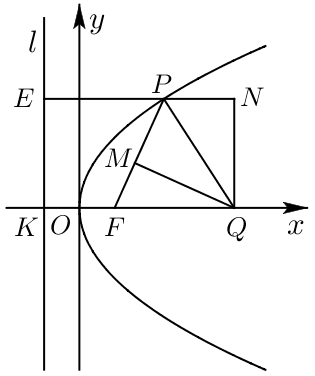
\includegraphics[width=30mm]{figs/16-拓10.png}}

\bindopt {\fontsize{10.5pt}{\qpTJgLeadLiti}\selectfont \makebox[\dimexpr0.5\linewidth-1em\relax][l]{A．\(|PE|=|PF|\)}\makebox[\dimexpr0.5\linewidth-1em\relax][l]{B．\(|PF|=|QF|\)}\par}

\bindopt {\fontsize{10.5pt}{\qpTJgLeadLiti}\selectfont \makebox[\dimexpr0.5\linewidth-1em\relax][l]{C．\(|PN|=|MF|\)}\makebox[\dimexpr0.5\linewidth-1em\relax][l]{D．\(|PN|=|KF|\)}\par}

{\ansblockgrayfalse
\begin{ansblock}[2章-拓-课时16-10]
% ans:2章-拓-课时16-10
\ansitem{39}{ABD}
\ansnote{详解}{A：由定义，\(|PF|\) 等于 \(P\) 到准线 \(l\) 的距离，而 \(PE\perp l\) 于 \(E\)，故 \(|PE|=|PF|\)，对．B：\(PQ\) 平分 \(\angle EPF\) 的外角，得 \(\angle FPQ=\angle NPQ\)；又 \(EN\parallel x\) 轴（同垂直于准线），故 \(\angle NPQ=\angle PQF\)（内错角），得 \(\angle FPQ=\angle PQF\)，\(\triangle FPQ\) 中 \(|PF|=|QF|\)，对．C：若 \(|PN|=|MF|\)，又 \(|QM|=|QN|\)（\(Q\) 在外角平分线上，到角两边等距）、\(\angle QMF=\angle QNP=90^{\circ}\)，则 \(\triangle FMQ\cong\triangle PNQ\)，得 \(|FQ|=|PQ|\)，结合 B 得 \(\triangle PFQ\) 为正三角形、\(\angle PFQ=\pi/3\)，则 \(P\) 被锁定为定点，与「\(P\) 为异于 \(O\) 的任意一点」矛盾，C 不恒成立．D：四边形 \(KQNE\) 为矩形（\(\angle KEQ=\angle EQN=\angle K=90^{\circ}\)），故 \(|EN|=|KQ|\)；\(|PN|=|EN|-|EP|=|KQ|-|PF|=|KF|+|FQ|-|PF|=|KF|\)（用 \(|EP|=|PF|=|FQ|\)），对．故选 ABD．}
\end{ansblock}}

\liB{变式\textbf{40}}{中档(知识点三)}{\duoxuan\hspace{0.6em}}{在平面直角坐标系 \(xOy\) 中，过抛物线 \(x^{2}=2y\) 的焦点的直线 \(l\) 与该抛物线的两个交点为 \(A(x_{1},y_{1})\)，\(B(x_{2},y_{2})\)，则\nobreak(\kongwei)}

\lxopt{A．抛物线在点 \(x=1\) 处切线方程为 \(2x-2y-1=0\)}

\lxopt{B．若点 \(M\) 坐标为 \((0,-1/2)\)，则 \(\overrightarrow{AM}\cdot\overrightarrow{BM}=0\)}

\lxopt{C．\(|OA|+|OB|>\sqrt{5}\)}

\lxopt{D．若 \(BN\) 垂直抛物线准线于点 \(N\)，则 \(A\)，\(O\)，\(N\) 三点在一条直线上}

{\ansblockgrayfalse
\begin{ansblock}[2章-拓-课时16-14]
% ans:2章-拓-课时16-14
\ansitem{40}{AD}
\ansnote{详解}{抛物线 \(x^{2}=2y\) 的焦点 \((0,1/2)\)、准线 \(y=-1/2\)．设 \(l\)：\(y=kx+1/2\)，代入 \(x^{2}=2y\) 得 \(x^{2}-2kx-1=0\)，\(x_{1}+x_{2}=2k\)、\(x_{1}x_{2}=-1\)；\(y_{1}+y_{2}=k(x_{1}+x_{2})+1=2k^{2}+1\)、\par\noindent \(y_{1}y_{2}=(kx_{1}+1/2)(kx_{2}+1/2)=k^{2}x_{1}x_{2}+(k/2)(x_{1}+x_{2})+1/4=-k^{2}+k^{2}+1/4=1/4\)．\par\noindent A：过点 \((1,1/2)\)、斜率 \(t\) 的直线 \(y=t(x-1)+1/2\) 代入 \(x^{2}=2y\) 得 \(x^{2}-2tx+2t-1=0\)，即 \((x-1)(x-(2t-1))=0\)，另一交点横标 \(2t-1\)；相切等价于 \(2t-1=1\)，即 \(t=1\)，切线 \(y=x-1/2\) 即 \(2x-2y-1=0\)，A 对．B：\(\overrightarrow{AM}\cdot\overrightarrow{BM}=(-x_{1},-1/2-y_{1})\cdot(-x_{2},-1/2-y_{2})=x_{1}x_{2}+(1/2+y_{1})(1/2+y_{2})=x_{1}x_{2}+1/4+(1/2)(y_{1}+y_{2})+y_{1}y_{2}=-1+1/4+(1/2)(2k^{2}+1)+1/4=k^{2}\)，仅 \(k=0\)（通径位）时为 0，不恒成立，B 错．C：取 \(l\parallel x\) 轴（\(k=0\)，即通径），\(A(1,1/2)\)、\(B(-1,1/2)\)，\(|OA|=|OB|=\sqrt{1+1/4}=\sqrt{5}/2\)，\(|OA|+|OB|=\sqrt{5}\)，严格不等式不成立，C 错．D：\(BN\perp\) 准线，得 \(N(x_{2},-1/2)\)；直线 \(OA\)：\(y=(y_{1}/x_{1})x=(x_{1}/2)x\)（用 \(y_{1}=x_{1}^{2}/2\)），代入 \(x=x_{2}\) 得纵标 \((x_{1}x_{2})/2=-1/2\)，即直线 \(OA\) 恰过 \(N(x_{2},-1/2)\)，\(A\)、\(O\)、\(N\) 共线，D 对．故选 AD．}
\end{ansblock}}

\liB{变式\textbf{41}}{简单(知识点三)}{}{已知点 \(P\) 在抛物线 \(y^{2}=-4x\) 上，求点 \(P\) 到椭圆 \(x^{2}/16+y^{2}/15=1\) 左顶点的距离最小值．}
\xiexwei{7mm}

\begin{ansblock}[2章-拓-课时16-20]
% ans:2章-拓-课时16-20
\ansitem{41}{2√3}
\ansnote{详解}{椭圆左顶点 \((-4,0)\)．设 \(P(-y^{2}/4,y)\)，则 \par\noindent \(d^{2}=(-y^{2}/4+4)^{2}+y^{2}=(1/16)y^{4}-y^{2}+16=(1/16)(y^{2}-8)^{2}+12\geqslant 12\)，\par\noindent 当 \(y^{2}=8\)（\(y=\pm 2\sqrt{2}\)，\(x=-2\)，点 \(P(-2,\pm 2\sqrt{2})\) 在抛物线上，核相符）时取等，\(d\) 的最小值为 \(\sqrt{12}=2\sqrt{3}\)．}
\end{ansblock}

\tjdnr{五}{拓展·轨迹方程与综合收难}{例\textbf{42}}{简单(知识点一)}{已知直线 \(l\)：\(x=-2\) 和圆 \(C\)：\((x-3)^{2}+y^{2}=1\)．若圆 \(M\) 与直线 \(l\) 相切，与圆 \(C\) 外切，求圆 \(M\) 的圆心 \(M\) 的轨迹方程．}
\xiexwei{12mm}

{\ansblockgrayfalse
\begin{ansblock}[2章-拓-课时16-23]
% ans:2章-拓-课时16-23
\ansitem{42}{y²=12x}
\ansnote{详解}{设圆 \(M\) 半径为 \(R\)．\(\odot C\) 圆心 \(C(3,0)\)、半径 1，外切，得 \(|MC|=R+1\)；\(\odot M\) 与直线 \(x=-2\) 相切，即圆心 \(M\) 到 \(x=-2\) 的距离为 \(R\)，从而 \(M\) 到直线 \(x=-3\) 的距离为 \(R+1\)．于是动点 \(M\) 到定点 \(C(3,0)\) 的距离等于它到定直线 \(x=-3\) 的距离，轨迹是以 \(C\) 为焦点、\(x=-3\) 为准线的抛物线（定义）：\(p/2=3\)、\(p=6\)，标准方程 \(y^{2}=12x\)．（核验 \(x\geqslant 0\)：\(M\) 到 \(x=-3\) 距离 \(=\) 横坐标 \(+3=R+1>0\) 且 \(|MC|=R+1\geqslant 1>0\) 自洽．）}
\end{ansblock}}

\liB{变式\textbf{43}}{中档(知识点三)}{}{已知等腰梯形 \(ABCD\) 的顶点都在抛物线 \(y^{2}=2px\)（\(p>0\)）上，且 \(AB\parallel CD\)，\(|AB|=2\)，\(|CD|=4\)，\(\angle ADC=60^{\circ}\)，则点 \(A\) 到抛物线的焦点的距离是\kongbai{}．}
\xiexwei{7mm}

{\ansblockgrayfalse
\begin{ansblock}[2章-拓-课时16-25]
% ans:2章-拓-课时16-25
\ansitem{43}{7√3/12}
\ansnote{详解}{等腰梯形两底 \(AB\parallel CD\)，而抛物线上平行于 \(x\) 轴方向的弦（两交点同纵坐标）不存在（\(y^{2}=2px\) 单值），故两底必为垂直于 \(x\) 轴的弦：\(A\)、\(B\) 关于 \(x\) 轴对称，\(C\)、\(D\) 关于 \(x\) 轴对称．由 \(|AB|=2\) 得 \(y_{A}=1\)（取上半），由 \(|CD|=4\) 得 \(y_{D}=2\)．设 \(A(m,1)\)；腰与底夹角 \(\angle ADC=60^{\circ}\)，底铅直，故 \(DA\) 与铅直线夹 \(60^{\circ}\)，纵差 \(2-1=1\)，故横差 \(=\tan 60^{\circ}=\sqrt{3}\)，\(D(m+\sqrt{3},2)\)．两点在抛物线上：\(1=2pm\)、\(4=2p(m+\sqrt{3})\)，两式相减 \(3=2\sqrt{3}p\)，得 \(p=\sqrt{3}/2\)、\(m=1/(2p)=\sqrt{3}/3\)．由焦半径（例 36 结论）\(|AF|=m+p/2=\sqrt{3}/3+\sqrt{3}/4=7\sqrt{3}/12\)．}
\end{ansblock}}

\tjdnr{五}{拓展·轨迹方程与综合收难}{例\textbf{44}}{中档(知识点三)}{已知动圆 \(M\) 过点 \((2,0)\)，被 \(y\) 轴截得的弦长为 4．}

\bindp (1) 求圆心 \(M\) 的轨迹方程；

\bindp (2) 若 \(\triangle ABC\) 的顶点在 \(M\) 的轨迹上，且点 \(A\)、\(C\) 关于 \(x\) 轴对称，直线 \(BC\) 经过点 \(F(1,0)\)，求证：直线 \(AB\) 恒过定点．
\xiexwei{18mm}

{\ansblockgrayfalse
\begin{ansblock}[2章-拓-课时16-29]
% ans:2章-拓-课时16-29
\ansitem{44}{(1) y²=4x；(2) 直线 AB 恒过定点 (−1,0)}
\ansnote{详解}{(1) 设圆心 \(M(x,y)\)，圆过 \((2,0)\)，则半径\({}^{2}=(x-2)^{2}+y^{2}\)；被 \(y\) 轴截弦长 4，则半径\({}^{2}=x^{2}+2^{2}\)（半弦 2、弦心距 \(|x|\)）．两式相等：\((x-2)^{2}+y^{2}=x^{2}+4\)，整理得 \(y^{2}=4x\)．\par\noindent (2) 顶点在轨迹 \(y^{2}=4x\) 上．设 \(B(x_{1},y_{1})\)、\(C(x_{2},y_{2})\)，\(BC\) 过 \(F(1,0)\) 且不垂直于坐标轴，设 \(BC\)：\(x=ty+1\)：\(y^{2}-4ty-4=0\)，韦达得 \(y_{1}y_{2}=-4\)．由 \(A\)、\(C\) 关于 \(x\) 轴对称，\(A(x_{2},-y_{2})\)．设 \(AB\)：\(y=kx+m\)（\(k\neq 0\)）代入 \(ky^{2}-4y+4m=0\)，其两根为 \(y_{1}\)、\(-y_{2}\)：\(y_{1}\cdot(-y_{2})=4m/k\)，即 \(4=4m/k\)、\(m=k\)．故 \(AB\)：\(y=k(x+1)\)，对一切实有 \(k\) 恒过定点 \((-1,0)\)．}
\end{ansblock}}

\liB{变式\textbf{45}}{中档(知识点三)}{}{已知抛物线 \(C\)：\(x^{2}=2py\)（\(p>0\)）与圆 \(O\)：\(x^{2}+y^{2}=12\) 相交于 \(A\)，\(B\) 两点，且点 \(A\) 的横坐标为 \(2\sqrt{2}\)．\(F\) 是抛物线 \(C\) 的焦点，过焦点的直线 \(l\) 与抛物线 \(C\) 相交于不同的两点 \(M\)，\(N\)．}

\bindp (1) 求抛物线 \(C\) 的方程；

\bindp (2) 过点 \(M\)，\(N\) 作抛物线 \(C\) 的切线 \(l_{1}\)，\(l_{2}\)，\(P(x_{0},y_{0})\) 是 \(l_{1}\)，\(l_{2}\) 的交点，求证：点 \(P\) 在定直线上．
\xiexwei{18mm}

{\ansblockgrayfalse
\begin{ansblock}[2章-拓-课时16-30]
% ans:2章-拓-课时16-30
\ansitem{45}{(1) x²=4y；(2) 点 P 恒在定直线 y=−1（即 C 的准线）上}
\ansnote{详解}{(1) \(A\) 横坐标 \(2\sqrt{2}\)、在圆上：\(y_{A}=(12-8)/2=2\)，\(A(2\sqrt{2},2)\)．代入 \(x^{2}=2py\)：\(8=4p\)、\(p=2\)，抛物线为 \(x^{2}=4y\)．\par\noindent (2) 先给切线式并验证：点 \(M(x_{1},x_{1}^{2}/4)\) 处，直线 \(y=(x_{1}/2)x-x_{1}^{2}/4\) 与 \(x^{2}=4y\) 联立得 \(x^{2}-2x_{1}x+x_{1}^{2}=(x-x_{1})^{2}=0\)，唯一公共点（重根 \(x_{1}\)），即为过 \(M\) 的切线 \(l_{1}\)；同理 \(N(x_{2},x_{2}^{2}/4)\) 处切线 \(l_{2}\)：\(y=(x_{2}/2)x-x_{2}^{2}/4\)．两切线联立：\((x_{1}-x_{2})x/2=(x_{1}^{2}-x_{2}^{2})/4\)，解得 \(x_{0}=(x_{1}+x_{2})/2\)，\(y_{0}=(x_{1}/2)x_{0}-x_{1}^{2}/4=x_{1}x_{2}/4\)．设 \(l\)：\(y=kx+1\)（过 \(F(0,1)\)；\(l\) 为 \(x=0\) 时与抛物线仅一交点，不合「不同两点」），代入 \(x^{2}=4y\)：\(x^{2}-4kx-4=0\)，故 \(x_{1}x_{2}=-4\)，故 \(y_{0}=-1\) 恒成立，点 \(P\) 恒在定直线 \(y=-1\)（准线）上．}
\end{ansblock}}

\xiaojie{①识别：垂线段中点、动圆切线、公共弦等轨迹方程问题与压轴综合收难，判归本题型.}
\bindp {\kaishu ②操作：轨迹题设参消参（或用定义直判焦点、准线），注明 \(x\geqslant 0\) 等范围与退化点；综合题先落标准形，再逐问拆解.}
\bindp {\kaishu ③收束：求证定点（定直线）要答出坐标（方程）；切线用联立重根验证，不引导数；收难题回代特位核对.}

% ============================================================
% 课堂评价 G5（恒5＝3单选+2填空＝导槽 G1~G5；ketang 新制顺排可跨栏，禁 \vbox 装栏）
% 印面号 46—50；多选门：本片正文多选 4（练01/拓08/拓10/拓14）≤4 合规
% ============================================================
\begin{ketang}{本组共5题（第46—50题），46—48为单选，49—50为填空．}

\jiancestem{{\fontsize{11.4pt}{14pt}\selectfont\heihao {\numboldjian 46}．}\hspace{4.1mm}\tieside{简单(知识点一)}\hspace{2.2mm}下列关于抛物线 \(y=2x^{2}\) 的图象描述正确的是\nobreak(\kongwei)}

\lxopt{A．开口向上，焦点为 \((0,1/8)\)}

\lxopt{B．开口向右，焦点为 \((0,1/8)\)}

\lxopt{C．开口向上，焦点为 \((0,1/2)\)}

\lxopt{D．开口向右，焦点为 \((0,1/2)\)}

\begin{ansblock}[2章-导-课时16-G1]
% ans:2章-导-课时16-G1
\ansitem{46}{A}
\ansnote{详解}{\(y=2x^{2}\) 即 \(x^{2}=(1/2)y\)，\(2p=1/2\)、\(p=1/4\)，开口向上，焦点 \((0,p/2)=(0,1/8)\)．故选 A．（验算：准线 \(y=-1/8\)，顶点 \((0,0)\) 到焦点、到准线等距 \(1/8\)，相符．）}
\end{ansblock}

\jiancestem{{\fontsize{11.4pt}{14pt}\selectfont\heihao {\numboldjian 47}．}\hspace{4.1mm}\tieside{简单(知识点一)}\hspace{2.2mm}抛物线 \(x^{2}=4y\) 的对称轴是直线\nobreak(\kongwei)}

\bindopt {\fontsize{10.5pt}{\qpTJgLeadPingjia}\selectfont \makebox[\dimexpr0.25\linewidth-0.5em\relax][l]{A．\(x=-2\)}\makebox[\dimexpr0.25\linewidth-0.5em\relax][l]{B．\(y=2\)}\makebox[\dimexpr0.25\linewidth-0.5em\relax][l]{C．\(y=0\)}\makebox[\dimexpr0.25\linewidth-0.5em\relax][l]{D．\(x=0\)}\par}

\begin{ansblock}[2章-导-课时16-G2]
% ans:2章-导-课时16-G2
\ansitem{47}{D}
\ansnote{详解}{\(x^{2}=4y\) 的焦点在 \(y\) 轴上，图象关于 \(y\) 轴对称，对称轴为直线 \(x=0\)．故选 D．（验算：点 \((2,1)\) 在曲线上（\(4=4\times 1\)，成立），其 \(y\) 轴对称点 \((-2,1)\) 亦在曲线上，相符；\(x\) 轴对称点 \((2,-1)\) 不在曲线上（\(4\neq -1\)）——对称轴确为 \(y\) 轴．）}
\end{ansblock}

\jiancestem{{\fontsize{11.4pt}{14pt}\selectfont\heihao {\numboldjian 48}．}\hspace{4.1mm}\tieside{简单(知识点三)}\hspace{2.2mm}若点 \(P\) 在抛物线 \(y^{2}=x\) 上，点 \(Q\) 在圆 \(M\)：\((x-3)^{2}+y^{2}=1\) 上，则 \(|PQ|\) 的最小值是\nobreak(\kongwei)}

\bindopt {\fontsize{10.5pt}{\qpTJgLeadPingjia}\selectfont \makebox[\dimexpr0.5\linewidth-1em\relax][l]{A．\(\sqrt{3}-1\)}\makebox[\dimexpr0.5\linewidth-1em\relax][l]{B．\(\sqrt{10}/2-1\)}\par}

\bindopt {\fontsize{10.5pt}{\qpTJgLeadPingjia}\selectfont \makebox[\dimexpr0.5\linewidth-1em\relax][l]{C．\(2\)}\makebox[\dimexpr0.5\linewidth-1em\relax][l]{D．\(\sqrt{11}/2-1\)}\par}

{\ansblockgrayfalse
\begin{ansblock}[2章-导-课时16-G3]
% ans:2章-导-课时16-G3
\ansitem{48}{D}
\ansnote{详解}{对圆上一点 \(Q\)，\(|PQ|\geqslant|PM|-|MQ|=|PM|-1\)（\(M\) 为圆心），且当 \(P\)、\(Q\)、\(M\) 共线、\(Q\) 在线段 \(PM\) 上时取等．设 \(P(x_{0},y_{0})\) 在 \(y^{2}=x\) 上，则 \(x_{0}=y_{0}^{2}\)，圆心 \(M(3,0)\)：\par\noindent \(|PM|^{2}=(y_{0}^{2}-3)^{2}+y_{0}^{2}\)．令 \(t=y_{0}^{2}\)（\(t\geqslant 0\)）：\(|PM|^{2}=(t-3)^{2}+t=t^{2}-5t+9=(t-5/2)^{2}+11/4\geqslant 11/4\)，\par\noindent 故 \(|PM|_{\min}=\sqrt{11}/2\)（\(t=5/2\) 时取得，此时 \(y_{0}=\pm\sqrt{10}/2\)，\(P(5/2,\pm\sqrt{10}/2)\) 在抛物线上，核相符），从而 \(|PQ|_{\min}=\sqrt{11}/2-1\)，选 D．（验算：\(t=5/2\)：\(|PM|^{2}=(5/2-3)^{2}+5/2=1/4+5/2=11/4\)，成立；\(|PM|_{\min}=\sqrt{11}/2>1\)，圆内不含抛物线点，\(|PQ|=|PM|-1\) 恒正、等号可取，核成立．）}
\end{ansblock}}

\jiancestem{{\fontsize{11.4pt}{14pt}\selectfont\heihao {\numboldjian 49}．}\hspace{4.1mm}\tieside{简单(知识点一)}\hspace{2.2mm}已知抛物线 \(y=(1/2)x^{2}\) 上距离点 \(A(0,a)\)（\(a>0\)）最近的点恰好是其顶点，则 \(a\) 的取值范围是\kongbai{}．}
\xiexwei{7mm}

{\ansblockgrayfalse
\begin{ansblock}[2章-导-课时16-G4]
% ans:2章-导-课时16-G4
\ansitem{49}{0<a≤1}
\ansnote{详解}{设 \(P(x,y)\) 为抛物线上任意一点，则 \(y=x^{2}/2\)（\(y\geqslant 0\)）．\par\noindent \(|AP|^{2}=x^{2}+(y-a)^{2}=2y+(y-a)^{2}=y^{2}+2(1-a)y+a^{2}\)．\par\noindent 这是关于 \(y\) 的二次函数，对称轴 \(y=a-1\)、开口向上．「最近点恰为顶点 \((0,0)\)」等价于 \(|AP|^{2}\) 在 \(y=0\) 处取最小值，等价于对称轴不在开区间 \((0,+\infty)\) 内、\(a-1\leqslant 0\)，故 \(a\leqslant 1\)．又 \(a>0\)，故 \(0<a\leqslant 1\)．（验算：\(a=1\)：\(|AP|^{2}=y^{2}+1\) 在 \(y=0\) 处最小，成立（顶点最近，边界值取得到）；\(a=1.1\)：对称轴 \(y=0.1>0\)，最近点非顶点，不合——故右端取闭，验证相符．）}
\end{ansblock}}

\jiancestem{{\fontsize{11.4pt}{14pt}\selectfont\heihao {\numboldjian 50}．}\hspace{4.1mm}\tieside{简单(知识点三)}\hspace{2.2mm}抛物线 \(y^{2}=4x\) 上的点到直线 \(x-y+4=0\) 的最小距离为\kongbai{}．}
\xiexwei{7mm}

{\ansblockgrayfalse
\begin{ansblock}[2章-导-课时16-G5]
% ans:2章-导-课时16-G5
\ansitem{50}{3√2/2}
\ansnote{详解}{设 \(P(t^{2}/4,t)\) 为抛物线上任意一点，则 \par\noindent \(d=|t^{2}/4-t+4|/\sqrt{1^{2}+1^{2}}=|t^{2}/4-t+4|/\sqrt{2}\)．\par\noindent 配方：\(t^{2}/4-t+4=(1/4)(t-2)^{2}+3>0\) 恒成立，故 \(d=(1/4)(t-2)^{2}/\sqrt{2}+3/\sqrt{2}\geqslant 3/\sqrt{2}=3\sqrt{2}/2\)，当 \(t=2\) 即 \(P(1,2)\) 时取得．（验算：\(P(1,2)\)：\(d=|1-2+4|/\sqrt{2}=3/\sqrt{2}=3\sqrt{2}/2\)，相符；联立 \(x=y^{2}/4\) 与直线得 \(y^{2}-4y+16=0\)，\(\Delta=16-64<0\)，直线与抛物线无公共点，最小值为正、在切点型位置取得，核成立．）}
\end{ansblock}}

\end{ketang}

% ---- 尾块（\tailfill 置 \end{multicols} 前；无参＝内容尾随框，件侧不擅自定高） ----
\tailfill

\end{multicols}
\end{document}
